%\documentclass[journal]{vgtc}                % final (journal style)
\documentclass[review,journal]{vgtc}         % review (journal style)
%\documentclass[widereview]{vgtc}             % wide-spaced review
%\documentclass[preprint,journal]{vgtc}       % preprint (journal style)
%\documentclass[electronic,journal]{vgtc}     % electronic version, journal

%% Uncomment one of the lines above depending on where your paper is
%% in the conference process. ``review'' and ``widereview'' are for review
%% submission, ``preprint'' is for pre-publication, and the final version
%% doesn't use a specific qualifier. Further, ``electronic'' includes
%% hyperreferences for more convenient online viewing.

%% Please use one of the ``review'' options in combination with the
%% assigned online id (see below) ONLY if your paper uses a double blind
%% review process. Some conferences, like IEEE Vis and InfoVis, have NOT
%% in the past.

%% Please note that the use of figures other than the optional teaser is not permitted on the first page
%% of the journal version.  Figures should begin on the second page and be
%% in CMYK or Grey scale format, otherwise, colour shifting may occur
%% during the printing process.  Papers submitted with figures other than the optional teaser on the
%% first page will be refused.

%% These three lines bring in essential packages: ``mathptmx'' for Type 1
%% typefaces, ``graphicx'' for inclusion of EPS figures. and ``times''
%% for proper handling of the times font family.

\usepackage{mathptmx}
\usepackage{graphicx}
\usepackage{times}

\usepackage{flushend}
\usepackage{subfigure}
\usepackage{amsmath}
\usepackage{amssymb}

\usepackage{vector}
\usepackage{algorithmic}
\usepackage{algorithm}

\renewcommand{\algorithmicrequire}{\textbf{Input:}}
\renewcommand{\algorithmicensure}{\textbf{Output:}}
\setlength\fboxsep{0pt}

%% We encourage the use of mathptmx for consistent usage of times font
%% throughout the proceedings. However, if you encounter conflicts
%% with other math-related packages, you may want to disable it.

%% If you are submitting a paper to a conference for review with a double
%% blind reviewing process, please replace the value ``0'' below with your
%% OnlineID. Otherwise, you may safely leave it at ``0''.
\onlineid{229}

%% declare the category of your paper, only shown in review mode
\vgtccategory{Algorithm/Technique}

%% allow for this line if you want the electronic option to work properly
\vgtcinsertpkg

%% In preprint mode you may define your own headline.
%\preprinttext{To appear in an IEEE VGTC sponsored conference.}

%% Paper title.

\title{Coherency-based Curve Compression\\ for Higher-Order Finite Element Model Exploration}

%% This is how authors are specified in the journal style

%% indicate IEEE Member or Student Member in form indicated below
\author{Alexander Bock, Erik Sund\'en, Bingchen Liu, Burkhard Wuensche, \textit{Member, IEEE}, and Timo Ropinski, \textit{Member, IEEE}}
\authorfooter{
%% insert punctuation at end of each item
\item
 Alexander Bock,  Erik Sund\'en and Timo Ropinski are with C-Research, Linkoping University E-mail: mr.t@imoropinski.com.
\item
 Bingchen Liu and Burkhard Wuensche is with Bioengineering Institute Engineering Science University of Auckland.
}

%other entries to be set up for journal
%\shortauthortitle{Biv \MakeLowercase{\textit{et al.}}: Global Illumination for Fun and Profit}
%\shortauthortitle{Firstauthor \MakeLowercase{\textit{et al.}}: Paper Title


%% Abstract section.
\abstract{Finite element (FE) models are frequently used in engineering and life sciences to represent the results of time-consuming simulations. In contrast to the regular grid structure facilitated by volumetric data sets, as used in medicine or geosciences, FE models are defined over a non-uniform grid. Elements can have curved faces and their interior can be defined through higher-order basis functions, which poses additional challenges when visualizing these models. During ray-casting the uniformly distributed sample points along each viewing ray must be transformed into the material space defined within each element. However, the computational complexity of this transformation makes a straight forward approach inadequate for interactive data exploration. In this paper, we introduce a novel coherence-based method which supports the interactive exploration of FE models by decoupling the expensive world-to-material space transformation from the rendering stage, thereby allowing it to be performed within a precomputation stage. Thus, it becomes possible to visually analyze higher-order FE models at interactive frame rates, even when they are time-varying or consist of multiple modalities. Within this paper, we provide the necessary background about the FE data, describe our decoupling method, and introduce our interactive rendering algorithm. Furthermore, we provide visual results and analyze the error introduced by the presented approach.} % end of abstract

%% Keywords that describe your work. Will show as 'Index Terms' in journal
%% please capitalize first letter and insert punctuation after last keyword
\keywords{Finite element visualization, GPU-based ray-casting.}

%% ACM Computing Classification System (CCS). 
%% See <http://www.acm.org/class/1998/> for details.
%% The ``\CCScat'' command takes four arguments.

\CCScatlist{ % not used in journal version
 \CCScat{I.3.7}{Computer Graphics}{Three-Dimensional Graphics and Realism}{Color, shading, shadowing, and texture}
}

%% Uncomment below to include a teaser figure.
\teaser{
	\centering 
  \subfigure[]{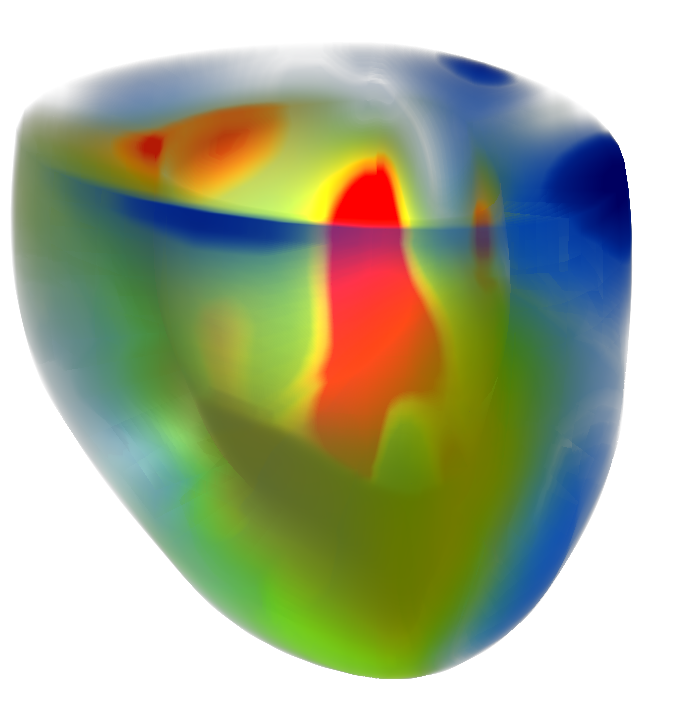
\includegraphics[width=0.2\linewidth]{figures/Heart1New1_T1}}
  \subfigure[]{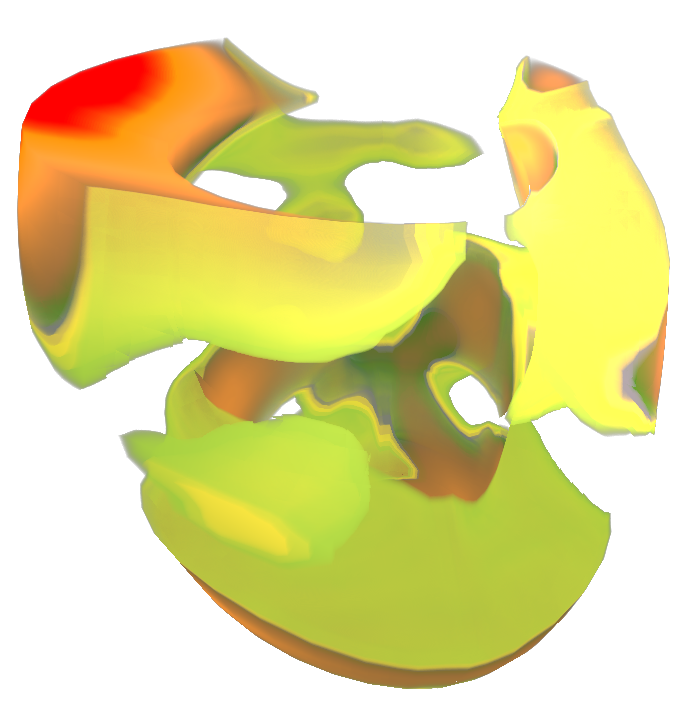
\includegraphics[width=0.2\linewidth]{figures/Heart1New2_T2}}
  \subfigure[]{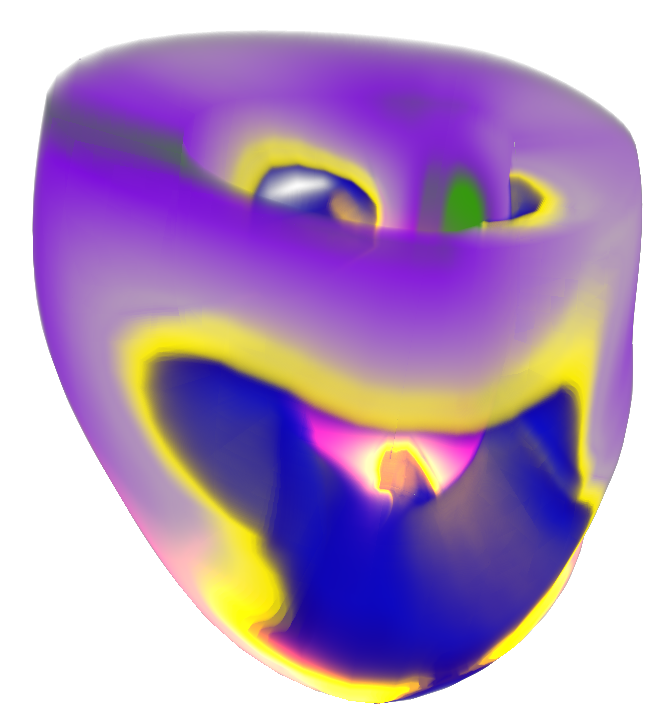
\includegraphics[width=0.2\linewidth]{figures/Heart4New1_T3}}
  \caption{Application of our visualization approach to a multi-parametric FE model of the left ventricle of a human heart. The images show volumetric renderings of different parameters defined over the FE model: minimum strain, medium strain and maximum strain ({\it left to right}). The data can be explored interactively by changing the transfer function and all other relevant rendering parameters.}
  \label{fig:heart}
}

%% Uncomment below to disable the manuscript note
%\renewcommand{\manuscriptnotetxt}{}

%% Copyright space is enabled by default as required by guidelines.
%% It is disabled by the 'review' option or via the following command:
% \nocopyrightspace

%%%%%%%%%%%%%%%%%%%%%%%%%%%%%%%%%%%%%%%%%%%%%%%%%%%%%%%%%%%%%%%%
%%%%%%%%%%%%%%%%%%%%%% START OF THE PAPER %%%%%%%%%%%%%%%%%%%%%%
%%%%%%%%%%%%%%%%%%%%%%%%%%%%%%%%%%%%%%%%%%%%%%%%%%%%%%%%%%%%%%%%%

\begin{document}

%% The ``\maketitle'' command must be the first command after the
%% ``\begin{document}'' command. It prepares and prints the title block.

%% the only exception to this rule is the \firstsection command
\firstsection{Introduction}\label{sec:introduction}

\maketitle

The finite element (FE) method is a computational technique frequently applied in science, medicine, and engineering to solve partial differential and integral equations~\cite{Young00}. The technique enables the discretization of complicated domains into arbitrarily shaped elements, in which material properties can be defined using nodal parameters and potentially higher-order interpolation functions. Thus, it becomes possible, to incorporate material properties at every point rather than a limited number of sample points. Applications include simulations of physical processes, e.\,g.,~disease processes, derivation of new entities from measured data, e.\,g.,~computation of material strain from displacement data, and analysis and comparison of data defined over objects with similar topology. All of these applications involve large amounts of multi-dimensional and multi-parametric data defined over arbitrarily shaped grid structures. A prominent application example from bioengineering, where FE visualization is essential, is the strain analysis of the human heart. An understanding of the full 3D strain tensor, represented by a symmetric matrix at each point, is necessary to identify unusual deformation behavior of the heart muscle and detect common patterns indicating developing diseases. Since there is little knowledge available about the exact behavior, interactive exploration plays an important role in the quest for new discoveries. While interactive surface-based visualizations of FE models are well established, volumetric visualization techniques supporting the interactive analysis of the entire 3D structure are rare~\cite{Wihelms90}. This is due to the fact, that accessing the materials defined over higher-order basis functions, which needs to be done for each sample in a volumetric visualization approach, involves high computational complexity. To avoid this computational complexity during the rendering stage of the visualization pipeline, FE models are often sampled to regular grids and rendered using standard volume rendering. However, this introduces errors, removes the relation between material geometry and material properties, and furthermore limits the resolution at which the data can be viewed. On top of this, resampling results in an extensive increase of the memory requirements, since it has to be performed for each parameter contained in a multi-parametric data set.

In this paper, we introduce an interactive volumetric ray-casting algorithm for FE models, which exploits the coherency of the curved viewing rays in order to reduce the computational complexity arising in the rendering stage. We exploit this coherency to precompute a view-independent proxy representation of the curved rays. To cope with the high number of proxy rays involved in this process, we apply curve clustering to compress the amount of data handled by our proxy ray data structure. This allows us to achieve interactive FE model visualization on modern graphics processing units (GPUs), and thus enables a true volumetric exploration of the entire FE model at interactive frame rates. Thus, we enable full volumetric and interactive exploration of potentially multi-parametric FE models, defined by higher-order basis functions, on a single GPU.

The paper is structured as follows. In the next section, we will describe previous work related to FE visualization. Section~\ref{sec:theory} explains the theory behind the FE data to be rendered, and Section~\ref{sec:preprocessing} describes the concepts underlying the data processing as well as the data layouts of the presented visualization approach. Section~\ref{sec:rendering} discusses the actual GPU-based ray-casting, and in Section~\ref{sec:results} we describe the achieved results, before concluding the paper in Section~\ref{sec:conclusions}.



\section{Related Work}\label{sec:relatedwork}

The FE method has several visualization related applications, such as the fitting of data to complex geometries, e.\,g., for strain computation from tagged MRI images~\cite{Young00}, surgical simulation~\cite{Berkley04} and breast image registration~\cite{lee10deformation}. In such applications the usage of curvilinear elements is popular, since they enable an appropriate modeling of these complex shapes~\cite{gelberg90visTechGrid,smith05ventricularmechanics}. However, interactive high-quality rendering incorporating the interior of the elements, is a demanding task. Often, the elements are resampled to lie in a common regular uniform grid~\cite{Wihelms90}. While this allows a direct visualization using standard volume rendering algorithms, it results in sampling-based errors as well as a loss of the material boundaries. Furthermore, resampling of multi-variate data sets would result in a vast data increase, which would need to be accessible during rendering. Furthermore, the loss of the material coordinate system information, which goes hand in hand with resampling, is a major drawback in many engineering applications where the interpretation of a field value only makes sense relative to the underlying material geometry, e.\,g., flow direction relative to the arterial wall or myocardial strain relative to the circumferential and radial direction of the ventricular muscle. As a consequence, many researchers have investigated rendering techniques which allow a more direct FE visualization by maintaining the relationship between the world and the material coordinate system. Wuensche introduced an isosurface-based approach for the visualization of biomedical tensor field data~\cite{wunsche03femvis}, which has been applied for strain analysis. Rose and Ertl propose a texture-based mesh reduction approach in order to render surface representations of large FE models at interactive frame rates~\cite{rose03femvis}. Other authors propose algorithms, which exploit a conversion into a tetrahedral mesh representation~\cite{marmitt05femtess,schroeder06femtess}. While these approaches can be considered as superior to resampling to a regular grid, they still prevent high accuracy. Alternatively, splatting-based approaches have also been applied~\cite{mao95femsplatting}, and view-independent point sampling strategies have been exploited to deal with higher-order data~\cite{zhou06pointbased}. To improve rendering quality, ray-casting approaches have been proposed. Garrity ~\cite{garrity90RaytracingIrregular} was the first to introduce ray-casting for rendering of unstructured meshes, thus suitable for FE models, by tracking numerous entry and exit points of a ray from the cells, which are stored in a hierarchical spatial data structure. Hong and Kaufman employ a projection of the elements' faces onto the image plane, to efficiently compute ray intersection points for the ray traversal~\cite{hong99curvilinear}. A similar strategy for finding intersection points is used by Farias et al., who apply a space sweeping approach~\cite{farias00zsweep}. Grimm et al. perform the intersection point computation on the GPU~\cite{grimm04curvilinear}. Their hybrid CPU/GPU approach performs a layer peeling on the GPU, while the actual ray-traversal is performed on the CPU. More recently, {\"U}ffinger et al. have presented a distributed visualization approach that allows volumetric visualization of models being defined through higher-order polynomials~\cite{uffinger10femraycasting}. Their approach is also based on ray-casting. However, in contrast to our approach, they circumvent computation of the world-to-material space transformation, by transforming the FE solution into a Cartesian reference space with barycentric coordinates. Then, the FE interpolation is replaced by a compact monomial representation, which the ray-casting kernel can use during sampling in physical space.



\section{Curvilinear Finite Element Models}\label{sec:theory}

While the presented concepts are in theory applicable to any FE model, they unfold their full potential when being applied to curvilinear FE models, where the material space is defined through higher-order basis functions. The curvilinear element examples presented in this paper employ cubic interpolation functions, whereby a tricubic element uses a 9-dimensional interpolation function, i.\,e., across the elements diagonal. Furthermore, to obtain optimal results, the number of elements should be moderate, as it is for instance the case in many application areas in bioengineering, e.\,g.,~\cite{lee10deformation} and \cite{wuensche03deformation}.

FE models are defined through two coordinate systems. First, the material or $\xi$ coordinate system, and second, the world coordinate system. The $\xi$ coordinate system is usually given in Cartesian coordinates and elements are represented using simple geometric shapes such as (unit) cubes or tetrahedra. The world coordinate system specifies the position and orientation of the elements in space by defining a set of nodal points. The dependent variables are almost always expressed in $\xi$ coordinates, since $\xi$ coordinates are independent of the element geometry, and thus support the analysis of multi-parametric data and the comparison of different FE models. Thus, the dependent variables and the FE interpolation functions are defined in $\xi$ space, while the nodal points are defined in world space. This combination allows to exploit the interpolation functions in order to compute variable values for all world space coordinates lying inside the model. More formally, the relation between $\xi$ and world coordinates can be expressed as follows. When we assume that each element $e_j$ is defined over the $[0,1]$ interval in $\xi$ space, i.\,e., $\xi(0)=x^{(e_j)}_1$ and $\xi(1)=x^{(e_j)}_2$, any point in the domain has a world coordinate $x$ with an associated $\xi$ coordinate. If the same basis functions $\phi_i$ are used for the geometry and the unknown variables, the mapping $x(\xi)$ is called isoparametric. However, in many practical applications, it is necessary to define associated material properties through higher-order interpolation functions.

\begin{figure}[t]
    \centering
    \subfigure[world space]{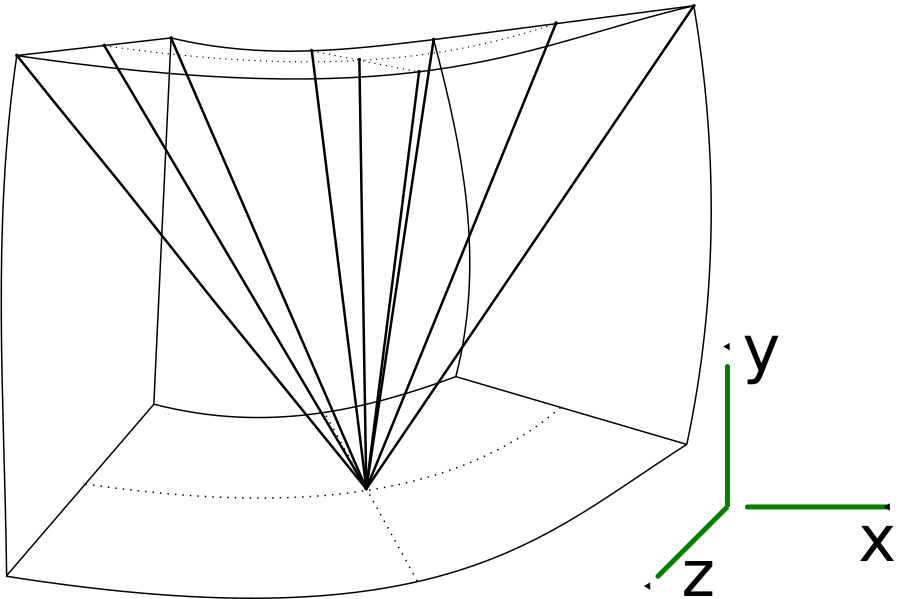
\includegraphics[width=0.4\linewidth]{figures/splines_world_space}}
    \hspace*{0.5cm}
    \subfigure[$\xi$ space]{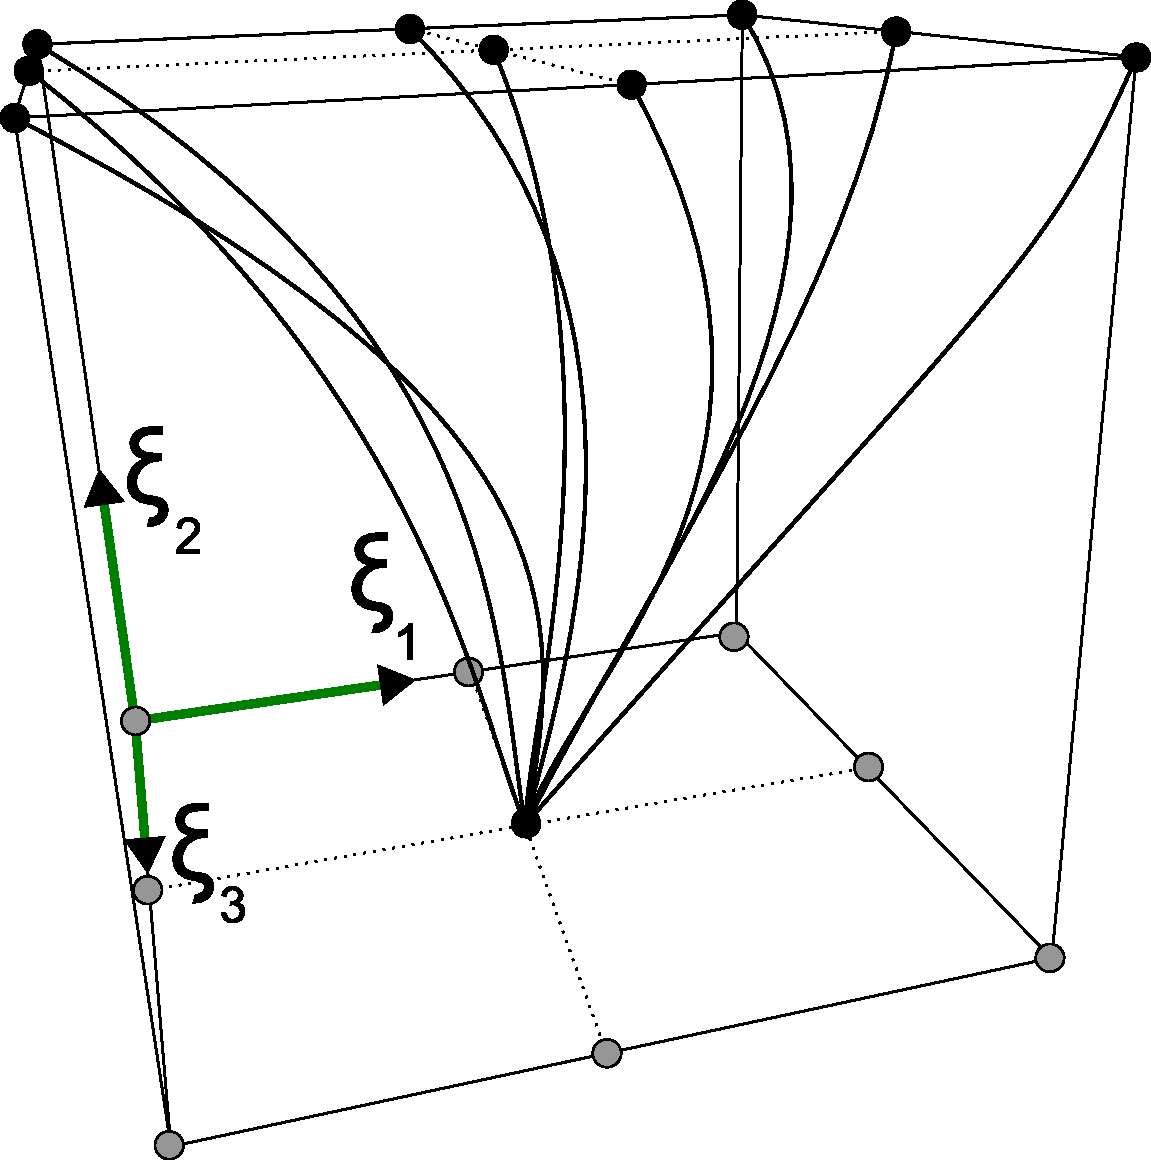
\includegraphics[width=0.4\linewidth]{figures/splines_xi_space}}
    \caption{When transforming straight rays given in world space ({\it a}) into $\xi$ space ({\it b}), these rays are bent and need to be represented as curves.}
    \label{fig:raycoords}
\end{figure}

When visualizing such models, world coordinates are usually more conveniently used, as they define the position and orientation of the elements. However, when a volumetric visualization is desired, $\xi$ coordinates need also be taken into account, as the dependent variables can only be accessed through $\xi$ space. Thus, the world coordinate system can be used for finding ray intersection points with the elements, while the actual ray traversal is performed in $\xi$ space. Thus, it is required to transform between the two coordinate systems during ray traversal. As it can be seen in Figure~\ref{fig:raycoords}, this transformation affects the geometry of the viewing rays, which end up as curves in $\xi$ space. While the transformation from $\xi$ space to world space can be computed fairly easy, as $x(\xi)=\sum_{i=1}^n x_i \phi_i(\xi)$, for $n$ nodal coordinates $x_i$, and basis functions $\phi_i$, the inverse transformation required during ray-casting is computationally much more demanding. Numerical methods, e.\,g., the multi-dimensional Newton method~\cite{Press92}, which are often applied to perform this transformation, involve high computational complexity and thus are not feasible in an interactive context. Therefore, alternative approaches are necessary to avoid the computational complexity of the world to $\xi$ space transformation in the rendering stage of the visualization pipeline.



\section{Coherency-based Curve Compression}\label{sec:preprocessing}

\begin{figure}[t]
    \centering
    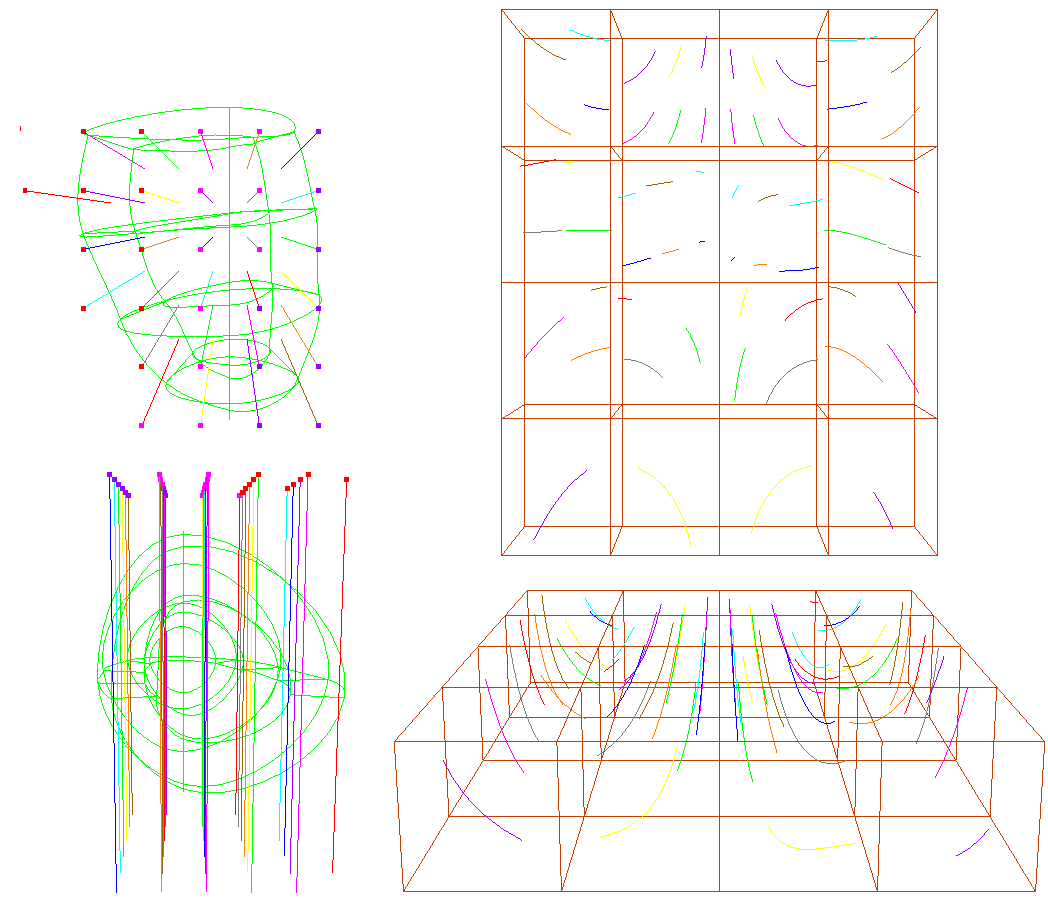
\includegraphics[width=0.95\linewidth]{figures/fem-crosscut.png}
    \caption{Rays which are adjacent in world space ({\it left}) have similar geometric properties in $\xi$ space ({\it right}). Color coding is applied to better allow the tracing of ray-segments as they intersect several elements in $\xi$ space.}
    \label{fig:coherency}
\end{figure}

In this section, we present the basis for a novel ray-casting based algorithm for the interactive exploration of curvilinear FE models. The straightforward approach for ray-casting FE models would be to march along a ray in world space and transform the world space sample coordinates $x$ into material coordinates $\xi$ before accessing the dependent variables. However, as discussed above, this approach is computationally very demanding and therefore cannot be performed at interactive frame rates. By using our approach, we are able to shift this originally view-dependent computation from the rendering stage into the data processing stage of the visualization pipeline. Thus, we can reduce the computation complexity necessary during rendering and achieve interactive frame rates when volume rendering curvilinear FE models. To perform the desired shift from the rendering stage into the data processing stage, we exploit the following key observations about the degree of coherency of curvilinear FE models. Finite Element method grids are designed to minimize approximation errors in the solution and to ensure convergence. In particular the Jacobian of the world-to-material coordinate mapping must be positive definite, and the grid resolution needs to be high enough that variations of the unknown variable can be adequately approximated with the underlying FE basis functions~\cite{knupp07meshquality}. This implicit smoothness constraint is exploited in our technique since it also limits the shape variations of neighboring rays in world coordinates mapped into material space, i.\,e., we can assume some degree of intra-element coherence. Because of the positive definiteness of the Jacobian we can employ the Newton method or similar solvers to compute the inverse of the material-to-world coordinate mapping at a point. Many FE applications require also some degree of inter-element compatibility, e.\,g., for the column problem involving axial deformations. Furthermore, many real-word objects have some degree of symmetry and self-similarity. These characteristics result in a FE mesh with clusters of similar elements and hence some degree of inter-element coherence. Figure~\ref{fig:coherency} illustrates this coherency, as it shows the shape of rays in $\xi$ space ({\it right}), which adjacently traverse world space ({\it left}). The element similarity is further demonstrated in the examples shown in Section~\ref{sec:results}.

\noindent In addition, coherence is supported, as most models in practical applications need {\it well-behaved} elements (low distortion and an aspect ratio close to one), in order to result in a stable numerical simulation. Consequently, we exploit inter- and intra-element coherence to reduce the computational complexity involved in ray-casting of FE models. The presented approach exploits precomputation, which is performed within two preprocessing steps as shown in Figure~\ref{fig:workflow}. In the first step, we compute a high number of proxy rays in $\xi$ space. These proxy rays act as a view- and resolution-independent spline representation of the actual viewing rays, which are cast through the material space during rendering. In the second step, we exploit inter- and intra-element coherence to reduce the vast number of proxy rays to a representative subset, which is the used during GPU-based ray-casting in the third step. By exploiting the precomputed data, which is independent of the used rendering parameters, FE models can be explored interactively by changing the transfer function and other rendering parameters. The following two subsections describe the two preprocessing steps, while the GPU-based ray-casting is discussed in Section~\ref{sec:rendering}.



\begin{figure*}[t]
    \centering
    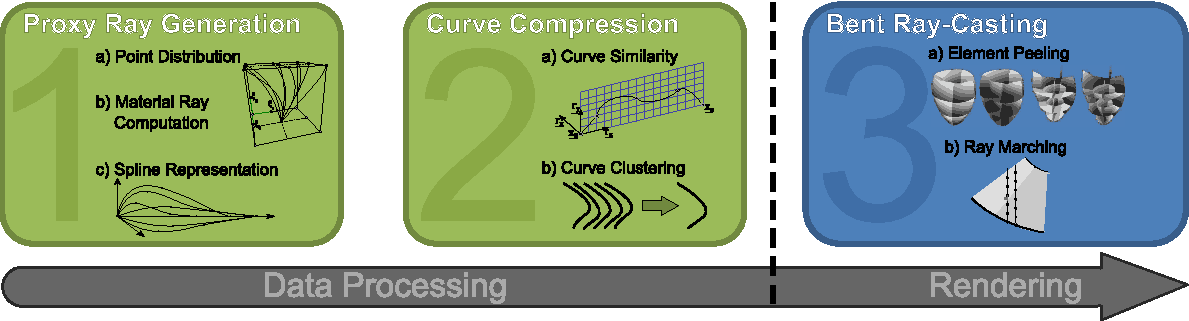
\includegraphics[width=0.8\textwidth]{figures/workflow-new.pdf}
    \caption{\textbf{Workflow.} To enable interactive ray-casting of curvilinear FE models, we exploit a multi-stage preprocessing approach. In the first step, we compute representative proxy rays, which are in the second step represented as splines and transformed into a common coordinate system. To reduce the data amount for the subsequent rendering stage, we apply a rotation invariant spline clustering in the third step. The resulting data, is then passed to the GPU-based rendering stage.}
    \label{fig:workflow}
\end{figure*}




\subsection{Proxy Ray Generation}\label{subsec:proxyraygeneration}

To be able to compute a complete set $R$ of proxy rays, it is essential that it covers all parts of the FE model. This means, that both, the world and the $\xi$ space, are densely populated with straight and curved rays, respectively. However, since the view direction used during rendering affects the ray traversal direction, it is not sufficient that all positions within an element are close to a proxy ray. They must also be close to proxy rays having different directions, which represent different viewing directions affecting the ray traversal. As the interpolation functions in $\xi$ space can be different for each element within one FE model, elements are treated individually during preprocessing and rendering. Finding the desired dense and omni directional proxy ray population for an element can be performed in two ways. It can be either done adaptively by analyzing the actual ray distribution within each element, or in a uniform way over each element. As our algorithm is based on the inter- and intra-element coherence, a uniform ray distribution is sufficient.

To obtain such a uniform proxy ray distribution we exploit the intra-element coherence, which results in a high similarity between rays in $\xi$ space which enter and exit an element through adjacent coordinates. Therefore, we compute a dense and uniform distribution $P$ of potential entry and exit points in $\xi$ coordinates on the surface of each element. While these points should be distributed over the entire surface of an element, the requirements with respect to the uniformity of $P$ are due to the intra-element coherence rather loose. We distribute the potential entry and exit points by performing an equidistant subdivision of all faces of an element. This is done for each element's face separately, by equidistantly subdividing the curved surface representing the face. In this step, the subdivision parameter $s_f$ controls the number of points equidistantly positioned along the $u$ and the $v$ coordinates of a face. Thus, the density of $P$ can be directly controlled by changing the subdivision parameter $s_f$. To reduce the number of initially generated proxy rays, it would also be an option to vary $s_f$ based on the extend of a face in world space. However, in cases where an element is strongly deformed, such that one face is much smaller than other faces, this usually indicates strong variations in the FE interpolation, which makes a higher sample density in world space necessary. Therefore, we have decided to choose a constant but sufficiently high $s_f$, before performing curve compression in the next step of our algorithm. This also results in a higher number of proxy rays, which is exploited in the coherency-based curve clustering.

The actual proxy rays are then computed based on the resulting point distribution $P$. To obtain proxy rays from $P$, we consider all pairwise combinations $(p',p'')$, with $p',p'' \in P$. During rendering, a ray intersecting $p'$ and $p''$ would be a line in world space and a curve in $\xi$ space (recall Figure~\ref{fig:raycoords}). When connecting $p'$ and $p''$ with a straight line, representing a viewing ray in world space, the proxy ray in $\xi$ space can be obtained by sampling along the line in world space and transforming each sample's position into $\xi$ space. While this sampling is performed with a fixed but sufficiently high sampling rate $s_r$, it should be pointed out, that it does not represent or determine the sampling rate used later on during rendering. $s_r$ is only used to obtain the geometry of the proxy rays, the sampling rate used for the compositing during ray-traversal in the rendering step can still be chosen freely.

As the set of proxy rays $R$ has to be dense, its size is obviously a limiting factor. Assuming that our subdivision parameter $s_f$ would result in $n$ distinct points along the $u$ and the $v$ coordinate of an element's face, we would have $n^2$ grid points on each face. Thus, we would have $n^2 \cdot f$ grid points in total, when considering that each element has $f$ faces. This would result in $r_u = (n^2 f)^2$ proxy rays to be precomputed. Though, we have kept $s_f$ constant to allow a less complex implementation of the ray-casting process, we have other possibilities to reduce the size of $R$. To achieve this reduction, we exploit properties of the standard volume rendering integral which is used in the rendering stage:

$$ L(x,\omega_o) = L_0 \cdot e^{-\int_{x_0}^{x}\kappa(x'')dx''} + \int_{x_0}^{x}  \! c(x') \cdot e^{-\int_{x'}^{x}\kappa(x'')dx''} dx'$$

\noindent where $c(x')$ represents the emissive color at sample $x'$ and $e^{-\int_{x_0}^{x}\kappa(x'')dx''}$ represents the exponential falloff between $x_0$ and $x$. When exploiting this rendering integral, the same observations hold as when applying the integral within the context of regular volume rendering. For a ray cast through a medium, the application of this integral results in an exponential falloff, i.\,e., when the ray is cast from one start point $x_0$ to one end point $x_n$ the samples in the regions surrounding $x_0$ will have considerable more influence on the image than those around $x_n$. In extreme cases, where structures with a high degree of opacity are rendered, samples close to $x_n$ do not have any influence at all. To select an optimal proxy ray subset during the precomputation stage, we take this observation into account. Therefore, we can use two different point distribution densities for entry and exit points, which is achieved by replacing $s_f$ with $s_f'$ and $s_f''$. Thus we obtain a point distribution of higher density, representing ray entry points, and a point distribution of lower density, representing exit points. Thus, when considering all entry and exit points of these two distributions in a pairwise manner, we achieve an importance-based ray sampling, where rays are more accurately represented when being close to the entry points. In comparison to the $r_u$ rays computed with the uniform proxy ray distribution, the importance-driven ray reconstruction approach results in $r_i = (n_{f} \cdot f) \cdot (n_{b} \cdot f)$ rays, where $n_{f}$ and $n_{b}$ represent the number of precomputed entry and exit points. This results in a decreased number of proxy rays, where the proxy ray set $R$ is more dense towards the respective end points and thus better complies with the exponential falloff which occurs during ray-casting.

As $s_f$ should be high but independent of the sampling rate used during rendering, it is unfeasible to store the proxy rays based on the precomputed samples. Again, with respect to the intra-element coherence, we can assume that the proxy rays in material space are well-behaved and are fairly continuous. Therefore, it is sufficient to store the proxy rays as parametric curves facilitating a lower number of control points than the original sampling density $s_f$. A spline is a parametric piecewise polynomial curve, which can be represented by bases for efficent computational use. Due to the requirements regarding interpolation of the control points, local control, numerical stability, and non-complex evaluation, Catmull-Rom splines~\cite{catmull74splines} are a natural choice for this parametric representation. Furthermore, Catmull-Rom splines have built-in $C^{0}$ and $C^{1}$ continuity, thus being continuous in position as well as tangent vector, which result in a smooth curve. Additionally, Catmul-Rom splines allow us to obtain and interpolate the start and end tangent of the curved rays directly.


\subsection{Curve Compression}\label{subsec:curvecompression}

The curve compression, which is used to obtain a manageable set of proxy rays during rendering, first reduces the number of proxy rays by exploiting orientation and scaling invariance, before computing a representative subset using clustering.

\noindent \textbf{Curve elimination.} In the previous subsection, we have described how to obtain a densely populated set of proxy ray curves, which are represented as parametric curves in $\xi$ space. As this set is obviously to large to be considered during rendering, we eliminate proxy rays from within this set, by taking into account the following three observations. First, a proxy ray does not have a pre-defined entry, exit point order. As the ray traversal and the compositing are performed in the rendering stage, we do not need to distinguish between two proxy rays with swapped entry and exit coordinates, if these are the same. The second helpful observation refers to the orientation of proxy rays in $\xi$ space. As a proxy ray represents only the traversal path, but not the dependent variables accessed during a traversal, we do not need to distinguish between two proxy rays which have the same overall geometry, but are differently oriented in $\xi$ space. As long as we know the entry and the exit point of a proxy ray, we can orient a proxy ray's geometry such that it is correctly oriented in $\xi$ space. This property is also related to the third observation, the arc length invariance, which we exploit to increase the similarity during curve compression. As soon as we know the coordinates of the entry and the exit points, we can not only adapt the orientation of a proxy ray, but also its scaling. Therefore, we do not have to distinguish between proxy rays, which have the same geometry when adapting the scaling factor along their principle axis.


\begin{figure}[b]
	\centering
	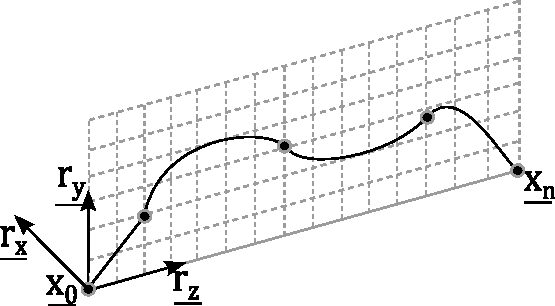
\includegraphics[width=0.75\linewidth]{figures/splinetransformation}
	\caption{To achieve a higher degree of similarity during the curve compression, we exploit the orientation invariance of the proxy rays and transform them into a common coordinate frame, where the principal curve axis coincidences with the $z$-axis. Furthermore, we exploit scale invariance to align all exit points.}
	\label{fig:proxyrayalignment}
\end{figure}


We exploit the three observations stated above, in order to achieve a higher degree of similarity during the subsequent clustering-based curve compression. To do so, we transform the parametric curves representing the proxy rays into a common coordinate frame, without compromising the uniqueness of each proxy ray curve. As proxy ray geometries are equal when their entry and exit points are equal, and as they comply to orientation and scaling invariance, we can transform all proxy rays into a common coordinate frame, where the entry and the exit point lie on the $z$-axis, such that the proxy ray curve's principal axis aligns with the same axis (see Figure~\ref{fig:proxyrayalignment}). To be further able to define the rotation around this axis, we take into account the first control point $c_i$ not being collinear with the start and the end point, and transform the proxy ray, such that $c_i$ it lies in the $yz$-plane. After this transformation $M_s$ has been applied, all proxy rays lie in the same coordinate frame as shown in Figure~\ref{fig:proxyrayalignment}, and thus the comparison performed during clustering reduces in a higher degree of similarity. While this transformation into a common coordinate frame reduces the number of rays, it requires us to store the angle of rotation $\theta$ for each proxy ray. This is necessary, as $\theta$ is required to be able to compute ${M_s}^{-1}$, which is needed during rendering to correctly orient the precomputed proxy rays.

\begin{figure*}[t]
    \centering
    \subfigure[entry world]{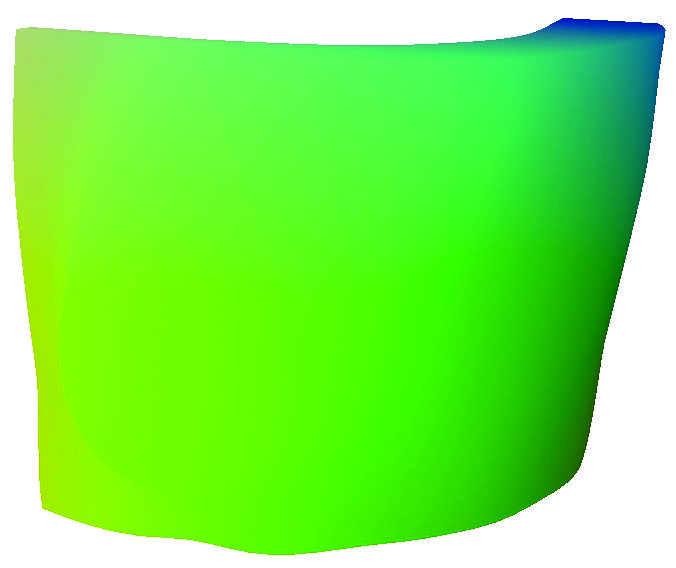
\includegraphics[width=0.15\linewidth]{figures/breast_mesh/BreastEntryWorld1}}
 	  \subfigure[entry depth]{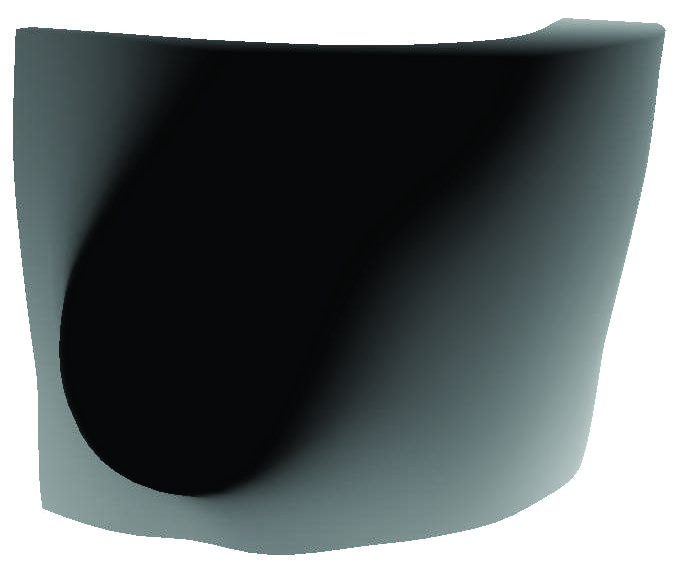
\includegraphics[width=0.15\linewidth]{figures/breast_mesh/BreastEntryDepth1}}
    \subfigure[entry $\xi$]{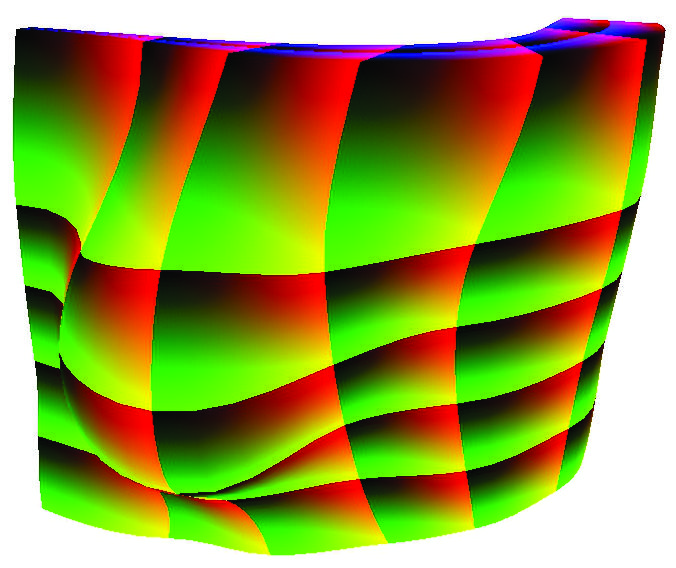
\includegraphics[width=0.15\linewidth]{figures/breast_mesh/BreastEntryXi1}}
    \subfigure[entry face IDs]{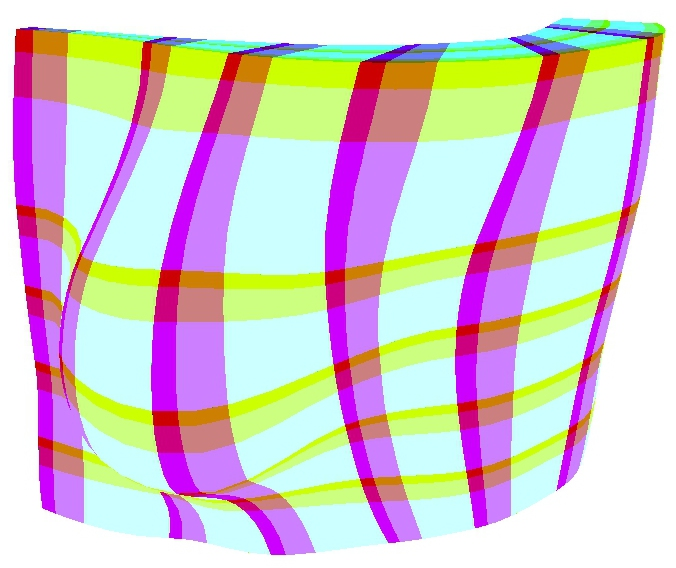
\includegraphics[width=0.15\linewidth]{figures/breast_mesh/BreastEntryFace1}}
    \subfigure[entry element IDs]{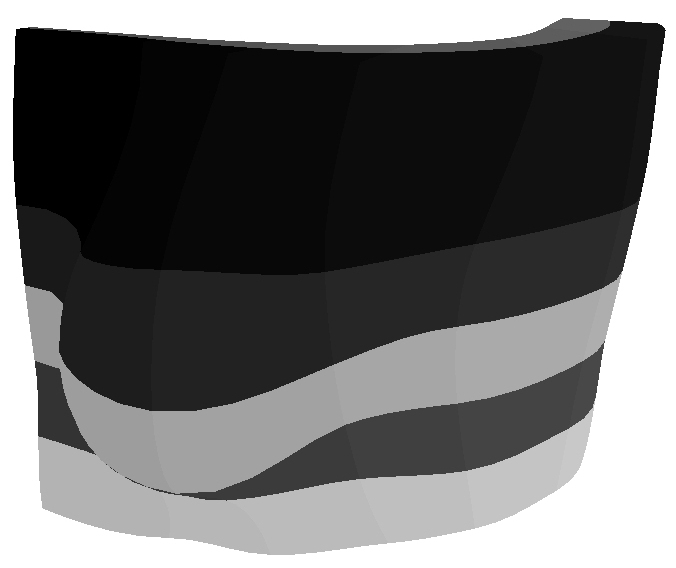
\includegraphics[width=0.15\linewidth]{figures/breast_mesh/BreastElementID1}}\\
    \subfigure[exit world]{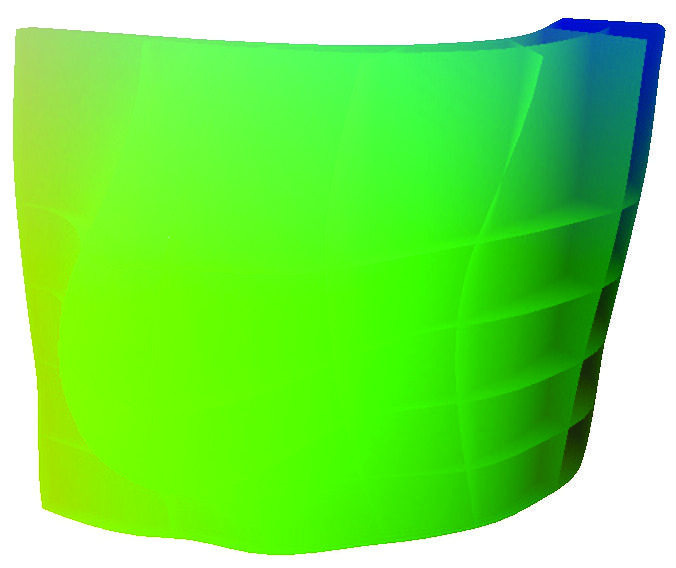
\includegraphics[width=0.15\linewidth]{figures/breast_mesh/BreastExitWorld1}}
 	  \subfigure[exit depth]{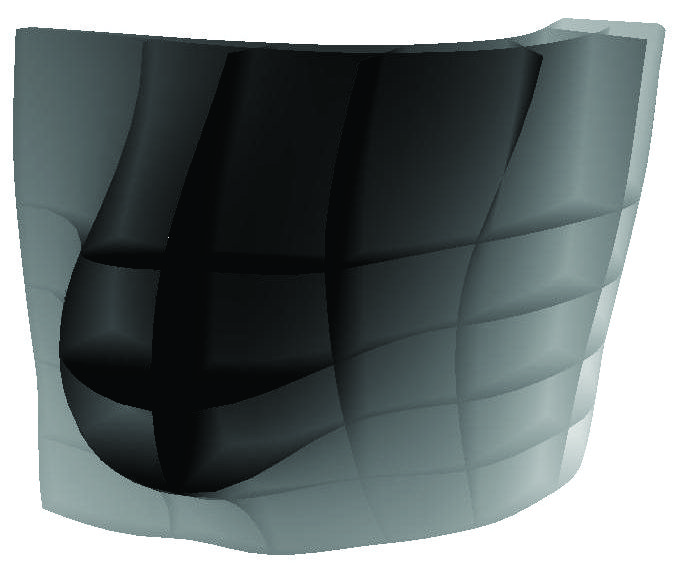
\includegraphics[width=0.15\linewidth]{figures/breast_mesh/BreastExitDepth1}}
    \subfigure[exit $\xi$]{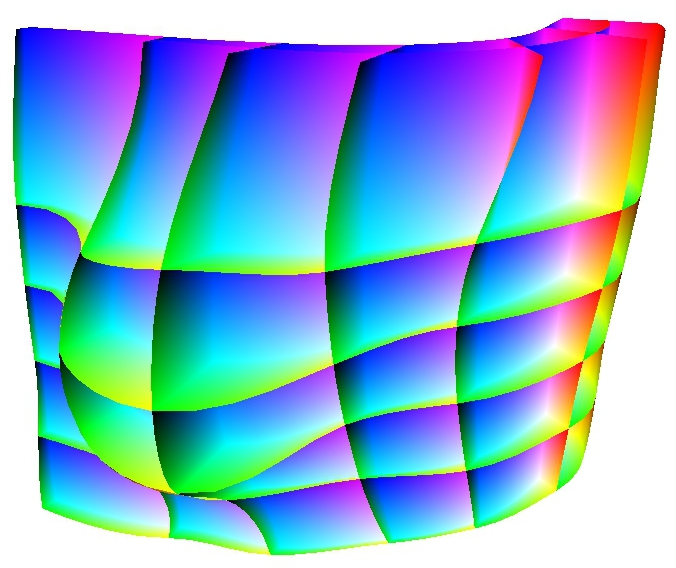
\includegraphics[width=0.15\linewidth]{figures/breast_mesh/BreastExitXi1}}
    \subfigure[exit face IDs]{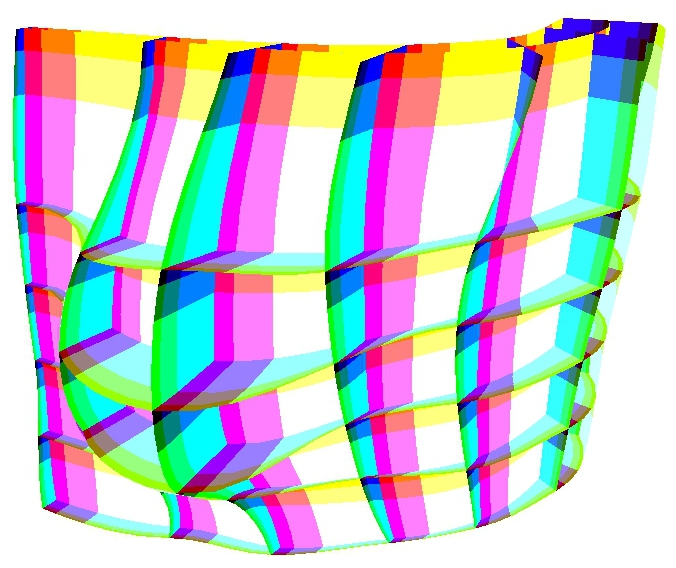
\includegraphics[width=0.15\linewidth]{figures/breast_mesh/BreastExitFace1}}
    \subfigure[exit element IDs]{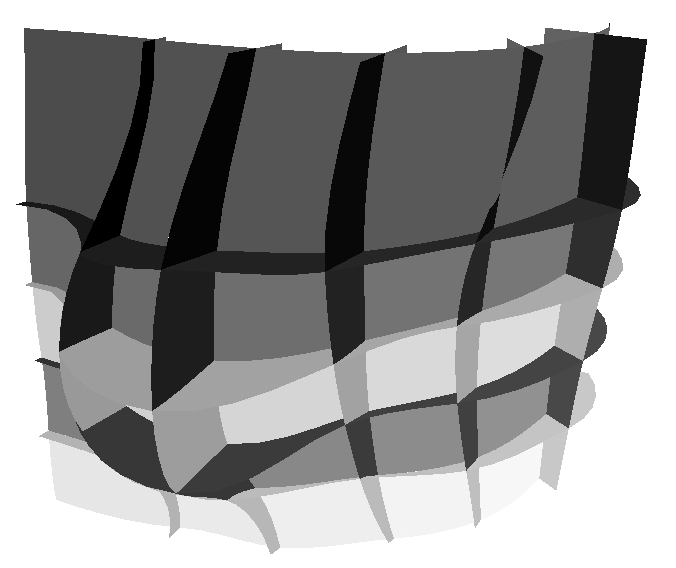
\includegraphics[width=0.15\linewidth]{figures/breast_mesh/BreastElementID2}}
    \caption{Depth peeling is used to extract the FE layers. The images show the world coordinates, its depth, the $\xi$ coordinate, the face ID and the element ID ({\it from left to right}), while the first row shows the first depth layer and the second row shows the second depth layer.}
    \label{fig:depthpeeling}
\end{figure*}


\noindent \textbf{Curve clustering.} While the curve elimination described above, already reduces the set $R$ of precomputed proxy rays, it is not sufficient to reduce it to a size manageable during rendering. To further reduce the size of $R$, we exploit the inter- and intra-element coherence discussed above. This allows us to perform clustering in order to obtain a representative subset of $R$. As several algorithms have been proposed for clustering curves, we have decided to exploit the approach proposed by Abraham et al.~\cite{abraham03clustering}. It has been originally developed for clustering functional data, that is represented through basis functions, which is a very similar setup as it exists in FE models. As this approach applies the clustering on the curve coefficients instead of the control points, it can be proven that the derived cluster representatives are optimal candidates. As we have previously reduced the set of proxy rays $R$ and increased curve similarity by transforming the proxy ray curves into a common coordinate frame, we can use a lower number of cluster representatives then when using a naive clustering approach. This reduces data size as well as computation time needed for the clustering. We will show how the number of clusters affects the achieved results in Section~\ref{sec:results}.

As Abraham et al. also state, the comparison metric used during the clustering is the most crucial part, as it directly defines the similarity of two curves~\cite{abraham03clustering}. Inspired by their work, we use the spanned area between two proxy ray curves as similarity metric. To compute the spanned area, we equidistantly sample the splines to be compared with a high sampling rate, and generate a triangle strip between the sampling points. The similarity can then be expressed by a Riemann sum of the triangle areas. If we have two proxy ray curves $a$ and $b$ with their sampled points $a_1,\dots,a_n$ and $b_1,\dots,b_n$, where due to the scale invariance $a_1=b_1$ and $a_n=b_n$ hold, we can calculate the approximate area between the splines. Let $x_iy_j$ denote the vector from $x_i$ to $y_j$, then the similarity of $a$ and $b$ is proportional to:

\begin{eqnarray*}
2\cdot d(x,y) &=& \Vert a_1a_2 \times a_2b_2\Vert + \\
&& \sum_{i=2}^{n-2}\Vert a_ia_{i+1} \times a_ib_i \Vert + \Vert b_ib_{i+1} \times b_{i+1}a_{i+1}\Vert + \\
&& \Vert a_{n-1}a_n \times a_{n-1}b_{n-1}\Vert,
\end{eqnarray*}

\noindent which equals twice the spanned area between $a$ and $b$, as the cross product will not give the area of the triangle itself, but the area of the parallelogram spanned by the two vectors. It is clear that this metric fulfills the metric traits of non-negativity, the identity of indiscernibles and symmetry, since all these properties hold for the area computation as well. For the actual clustering, we exploit the k-means clustering algorithm, which has been originally presented by Hartigan~\cite{hartigan75kmeans}. It has the benefits, that it is robust even with large high-dimensional data and only needs the number of final clusters and a metric as parameters. Unfortunately, the number of clusters is not known a-priori and, in fact, there might be no definite answer, which is the best number in general. To deal with this problem, we have evaluated the impact of different numbers of clusters in Section~\ref{sec:results}. Alternatively, one could apply algorithms for finding an optimal number of clusters, such as for instance k-fold cross-validation, which is often used together with k-means. As output, k-means provides the desired clusters with one representative proxy ray for each of them. Besides the obtained cluster representatives, we need to store for each proxy ray, specified by its entry and exit point, its cluster ID to associate it with the cluster it belongs to, as well as the $z$-axis angle $\theta$, which is used to exploit the orientation invariance.



\section{Bended Ray-Casting}\label{sec:rendering}
While Section~\ref{sec:preprocessing} gives a comprehensive overview of the preprocessing steps needed to obtain the proxy ray set $R$, the actual rendering process is discussed in greater detail within this section. We perform GPU-based ray-casting by exploiting the data generated during the preprocessing stage, i.\,e., a list storing the associated cluster ID as well as the $z$-axis rotation angle $\theta$ for each proxy ray. To be able to reconstruct the actual proxy ray geometry, we further need to have access to the cluster representatives. As the elements are treated individually, we need a way to be able to associate ray segments with the elements and connect them through compositing. Thus, the rendering stage is divided into three substages. First, element peeling which allows to obtain the entry and exit points for each element. Second, ray marching where a ray in $\xi$ space is reconstructed from the the preprocessed data before it is traversed. And third, ray interpolation which is used to be able to deal also with less dense proxy ray sets $R$. These three substages are discussed in the following three subsections.


\subsection{Element Peeling}

\begin{figure}[t]
  \centering
  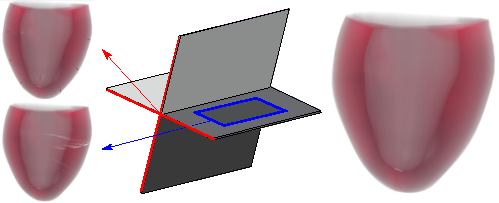
\includegraphics{figures/coincidence/Coincidence.pdf}
  \caption{Two cases of depth coincidence can occur, as illustrated ({\it middle}), when rendering adjacent polygons. Point coincidence occurs at the corners of adjacent elements ({\it top left}), while surface coincidence occurs at the touching element's surfaces ({\it bottom left}). All coincidences can be avoided ({\it right}).}  
  \label{fig:depthcoincidence}
\end{figure}


As the visualized FE models consist of several elements, these overlap in image space. Therefore, mechanisms are needed to determine, which sequence of proxy rays best represents a specific pixel. To obtain this sequence of proxy rays, we exploit a modified depth peeling approach~\cite{mammen89DepthPeeling}. With this approach, we can peel away layer-by-layer from the rendered FE model by using an additional depth comparison. However, when using depth peeling, it is crucial to be able to distinguish between different fragments solely based on their depth values. In order to deal with problems arising from fragments coinciding at the same depth value, often a user-defined bias parameter is introduced~\cite{Everitt01interactiveorder-independent}. As this coincidence of depth values is not the regular case and can be considered as rather rare compared to those fragments not coinciding in depth, the error introduced due to this bias is often neglectable, which makes it a common practice in many computer graphics applications. Unfortunately, in our case the situation is more severe. As a FE model exists of several adjacent, i.\,e., touching, elements, coinciding depth values are the norm and need to be handled robustly. As illustrated in Figure~\ref{fig:depthcoincidence}, two cases of depth coincidence occur. Point coincidences occur at the corners of adjacent elements~({\it a}) and surface coincidences occur where two adjacent element's surfaces are touching~({\it b}). Since semi-transparency is accumulated along the viewing rays, errors introduced by the bias would be prominent in the rendered image. Therefore, we have realized a multi-layer depth peeling, where we exploit information available in the form of several attributes to resolve the depth coincidences without introducing an error. Figure~\ref{fig:depthpeeling} shows the employed information next to the color coded $\xi$ and world space coordinates of the first two layers of a FE model. Besides the actual depth values, we take also into account the current element's ID, as well as the ID of the current surface in our peeling approach. Thus, we can resolve the described coincidence cases. In general we set the additional depth test to accept all fragments which have a greater or equal depth than the current fragment. To resolve the two coincidence cases, we ensure that each pair of entry- and exit-points has the same element ID. This together with ensuring that they have different face IDs, is enough to correctly resolve the point and the surface coincidence (see Figure~\ref{fig:depthcoincidence}).


\begin{figure}[b]
    \centering
    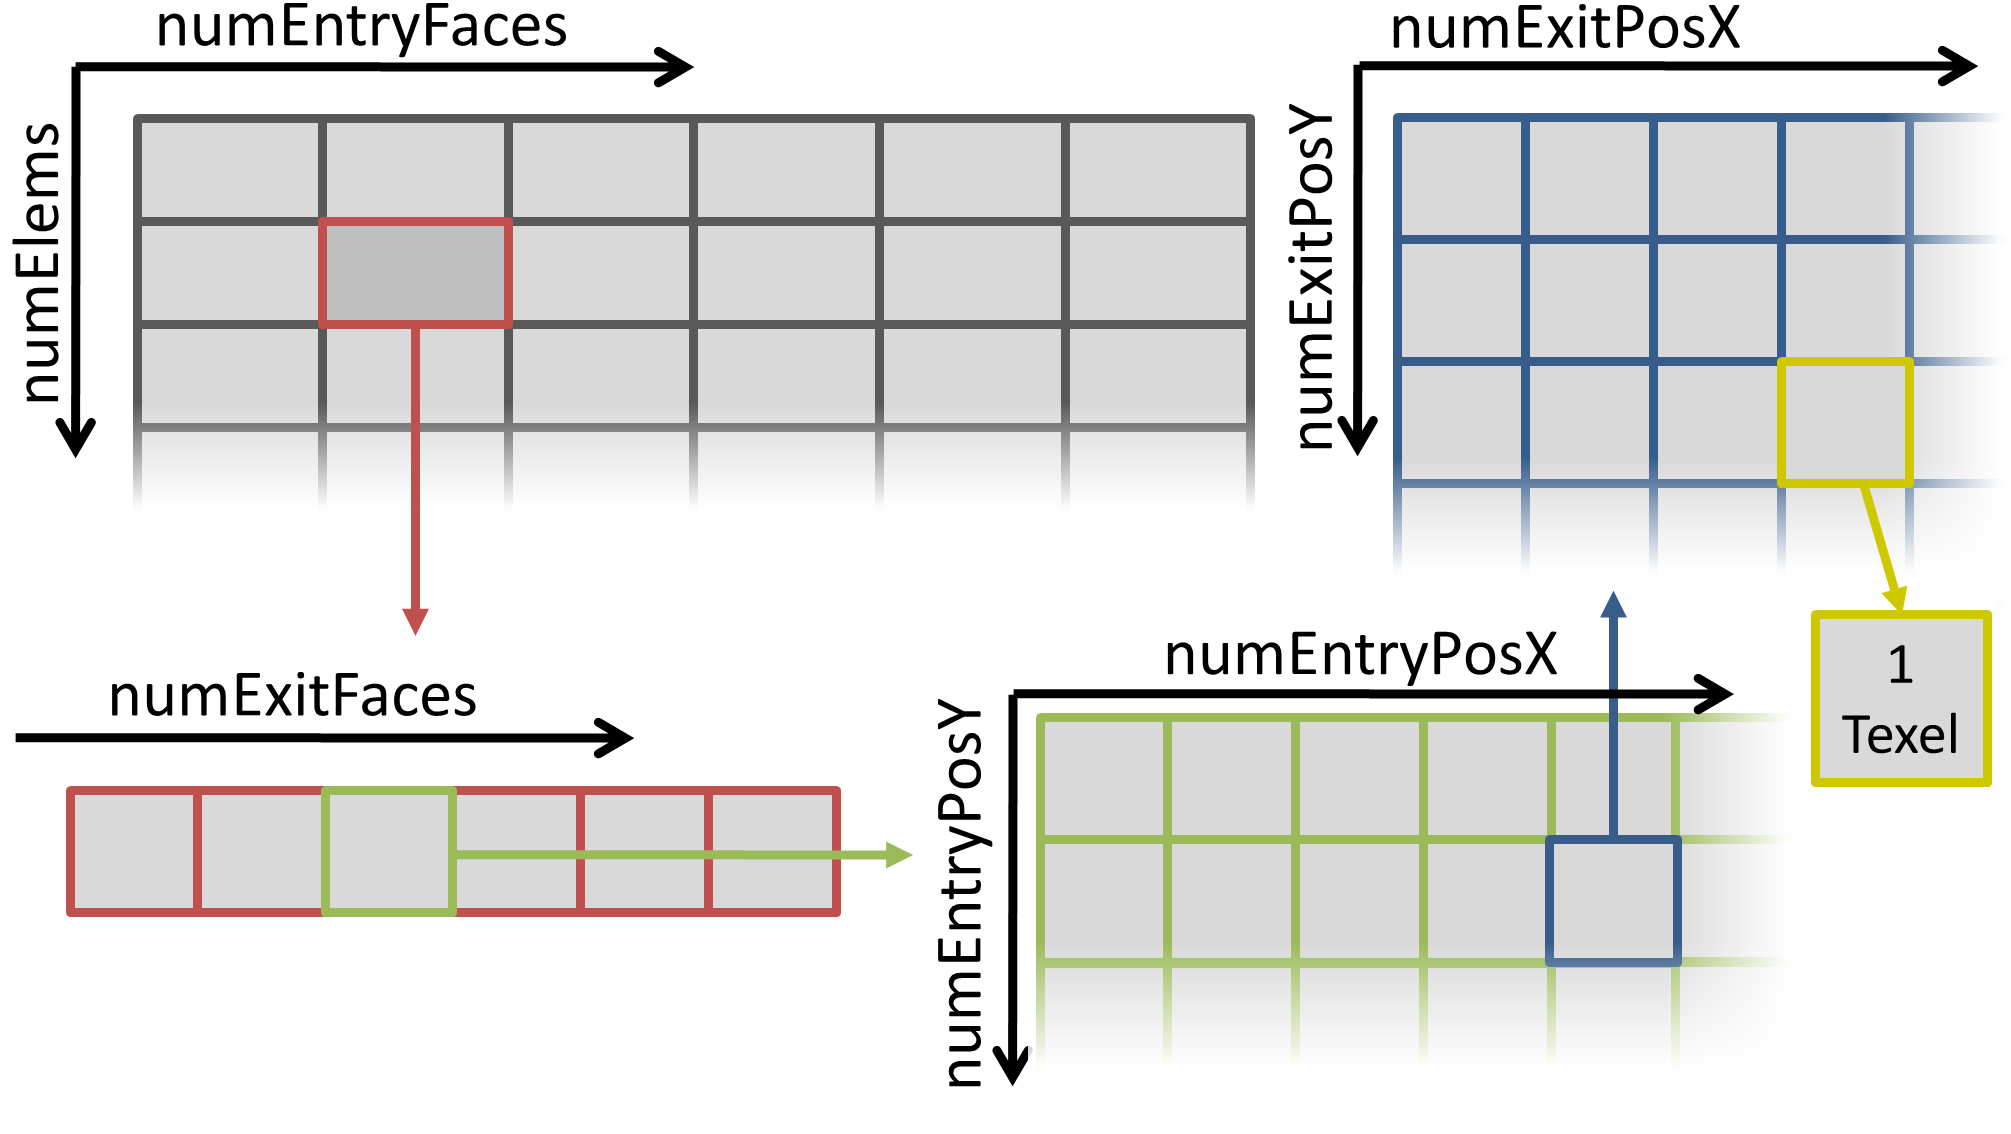
\includegraphics[width=\linewidth]{figures/curvetexmap-memorylayout}
    \caption{Memory layout used to gain access to the precomputed proxy ray information. To retrieve the information required during rendering in constant time, a hierarchical subdivision is exploited. For each proxy ray, we store the cluster ID as well as the rotation angle $\theta$.}
    \label{fig:memorylayout}
\end{figure}


As we also take into account the current face and element ID during depth peeling, we can use this information to obtain the precomputed values for each proxy ray. We know for each proxy ray segment the FE $c$ it is traveling through, the face $f_s$ through which it enters $c$ and the face $f_e$ through which it exits $c$. Having this information, we need to identify the precomputed values for the rays closest to the actual ray start point $s_{w_0}$ and its end point $s_{w_n}$. To achieve this in constant time, we exploit the memory layout illustrated in Figure~\ref{fig:memorylayout}. On the highest level of the hierarchy, we arrange the data based on $f_s$ along the $x$-axis and $c$ along the $y$-axis. Thus, we obtain $n_{cells} \cdot n_{faces}$ cells which contain the precomputed information for rays entering a FE $c$ through a specific face $f_s$. Each of these cells is partitioned based on the $f_e$ along the $x$-axis, such that the resulting cells contain only the information for those rays exiting through a specific face $f_e$. Now, we can identify such a cell based on $c$, $f_s$ and $f_e$. To be able to access the precomputed ray data for a ray entering $c$ through $f_s$ at $s_{w_0}$ and leaving through $f_e$ at $s_{w_n}$, we again partition the cells based on the number $n_{entry}$ of precomputed entry points per face. Finally the thus obtained cells are partitioned based on the number $n_{exit}$ of precomputed exit points per face. To access the data for a ray within this hierarchical memory layout, we require the patch coordinates of $s_{w_0}$ and $s_{w_n}$ in addition to $c$, $f_s$ and $f_e$. Thus, we can obtain the preprocessed proxy ray information, which is stored in texture memory on the GPU, by accessing the hierarchical data structure at position $p$:

\begin{eqnarray*}
p_x & = &(f_s \cdot (n_{entry} \cdot n_{exit} \cdot n_{cells})) + \\
	&  &(f_e \cdot (n_{entry} \cdot n_{exit})) + (s_{w_0,x} \cdot n_{exit}) + s_{w_n,x}\\
p_y & = &(c   \cdot (n_{entry} \cdot n_{exit})) + (s_{w_0,y} \cdot n_{exit}) + s_{w_n,y}
\end{eqnarray*}


\subsection{Ray Marching}

\begin{figure}[t]
\centering
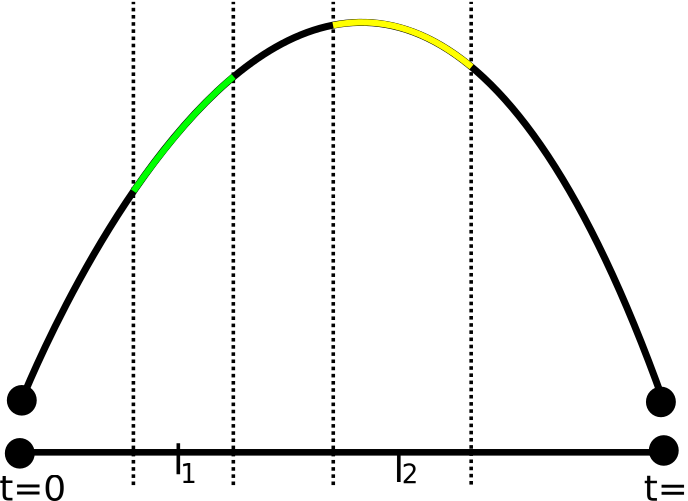
\includegraphics[width=0.5\linewidth]{figures/arclength}
\caption{To achieve equidistant sampling along a curve ray in $\xi$ space ({\it top}), an arc length parametrization is applied, resulting in a non-uniform sampling in world space ({\it bottom}).}
\label{fig:arclength}
\end{figure}

Once we know, which proxy ray information needs to be accessed in the hierarchy, we can reconstruct its ray geometry by retrieving the spline coefficients for the obtained cluster ID. The thus reconstructed spline is then transformed back from the canonical orientation along the $z$-axis, by applying ${M_s}^{-1}$, such the spline lies between the entry- and the exit-point of the actual viewing ray in world coordinates. Once the proxy ray curve has been transformed back into its originally location, we can march along it and perform the actual bended ray-casting by fetching the dependent variables from the $\xi$ space. However, we need to ensure that we have an equidistant sampling along the reconstructed ray in order to obtain optimal results. The splines, however, are parameterized by the parameter value $t \in [0,1]$ in world coordinates, which does not take the shape of the ray in $\xi$ space into account, e.\,g. given a spline $s$, $\Vert s(i) - s(j) \Vert \neq \Vert i - j \Vert$. That means that an equidistant sampling in world space will result in not equidistant sampling points along the curve in $\xi$ space. As illustrated in Figure~\ref{fig:arclength}, we address this problem by using an arc length parametrization as presented by Guenter and Parent~\cite{guenter90arclength}. This leads to a function $t \mapsto t'$. If the sampling is done using $t'$ instead of $t$, the sampled values will be equidistant along the curve in $\xi$ space.

\begin{figure}[b]
    \centering
    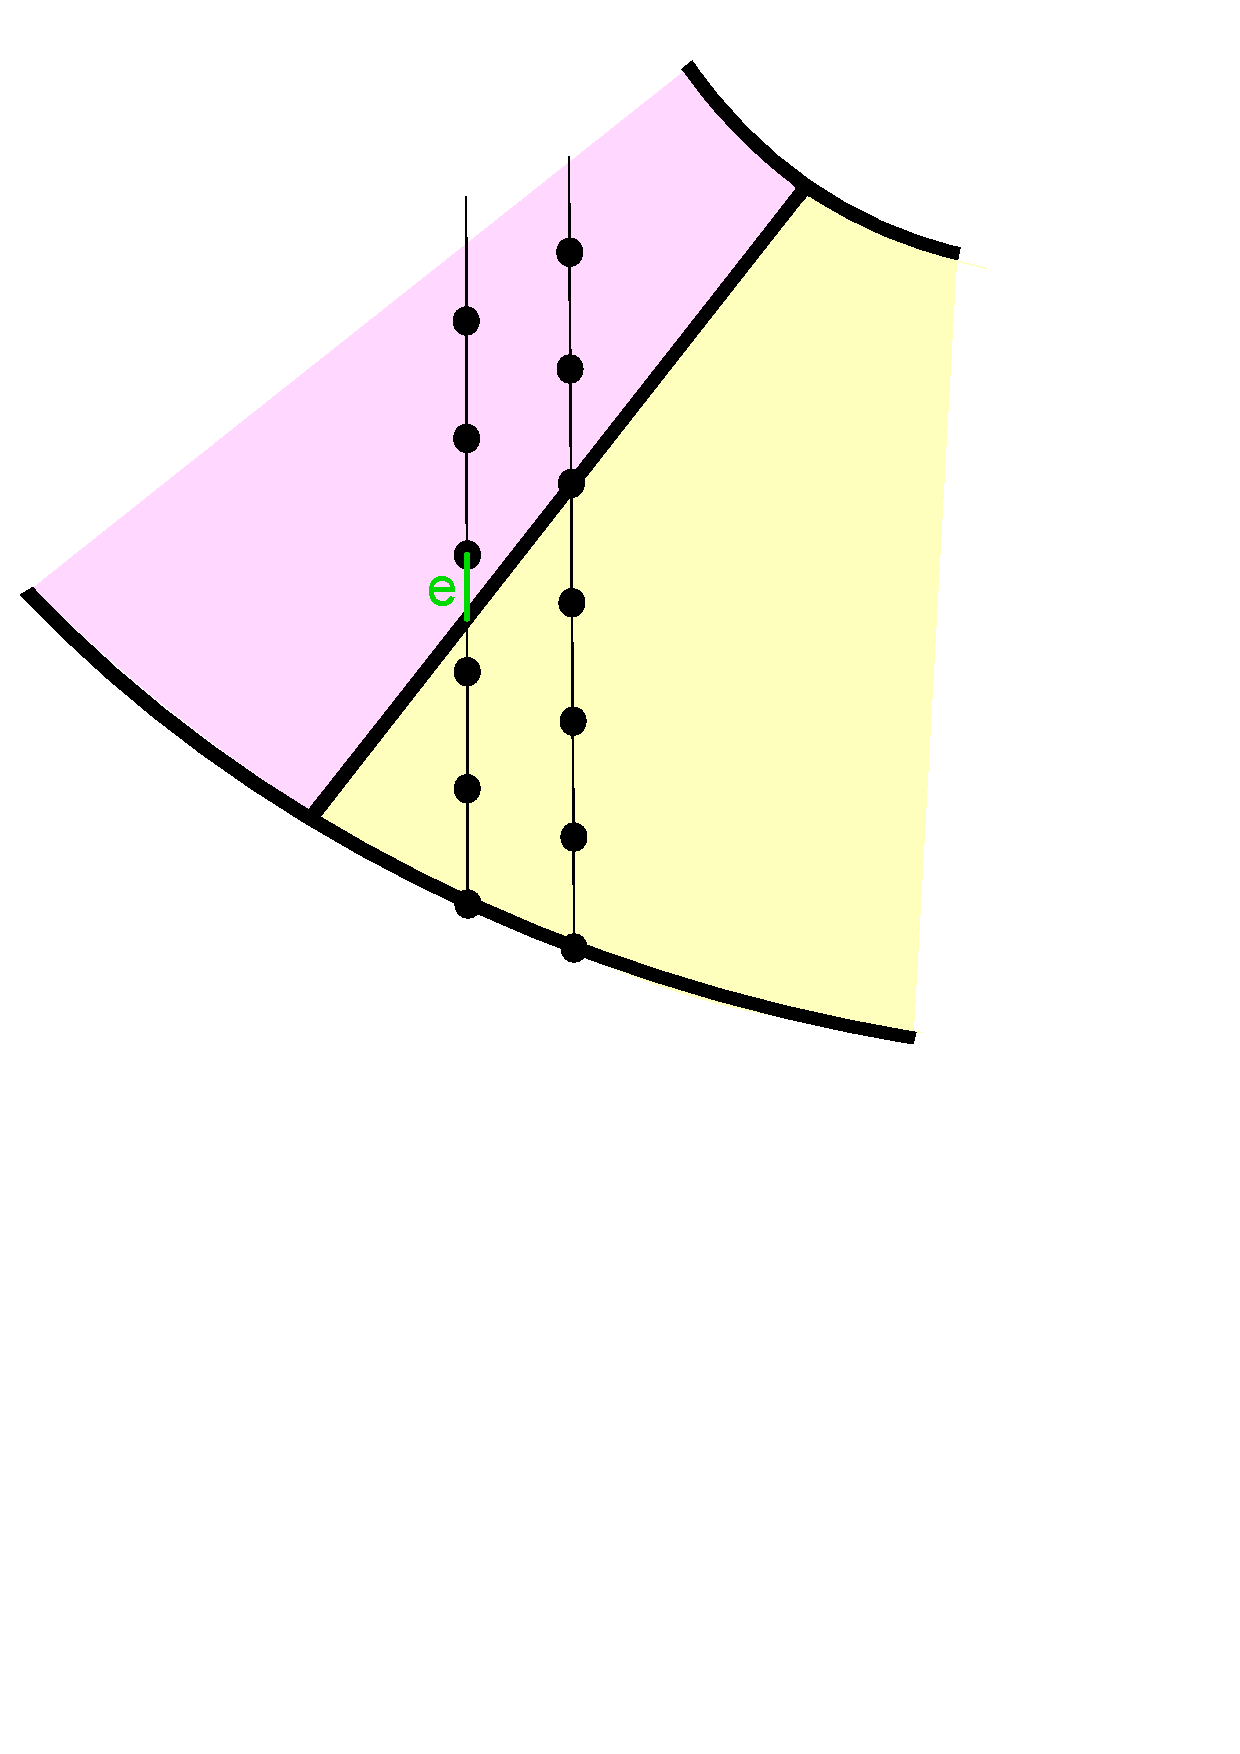
\includegraphics[width=0.3\linewidth]{figures/overshoot}
    \caption{Rays penetrating multiple elements must be processed, such that constant sampling step sizes are obtained at the borders. The overshoot $e$ of $FE_0$ can be used to offset the first sampling point in element $FE_1$.}
    \label{fig:overshoot}
\end{figure}

The subdivision of a curve ray penetrating the whole FE model into segments based on the penetrated FEs, requires an appropriate border handling scheme. If we sample the ray equidistantly in a naive way, the last point on the ray, which lies on the exit face of a FE, might not coincide with an intended sampling point (see Figure~\ref{fig:overshoot}). When we for instance consider a ray $a$ which is divided into two segments $r$ and $s$ in such a way that $r_n = s_0$, i.\,e., the last sample point of $r$ is the first sample point of $s$. In this situation, we would have an equidistant sampling rate of $\left|a_i - a_{i+1}\right| = \delta$ for the two rays. However, the naive implementation will have $\left|r_{n-1} - r_{n}\right| \neq \delta$. To remedy this, we do not sample the last point on each ray but save the overshoot instead and use it as an offset for the first sampling point in the next ray segment.



\subsection{Ray Interpolation}

\begin{figure}[t]
    \centering 
    \subfigure[$2 \times 2$ precomputed proxy rays per element]{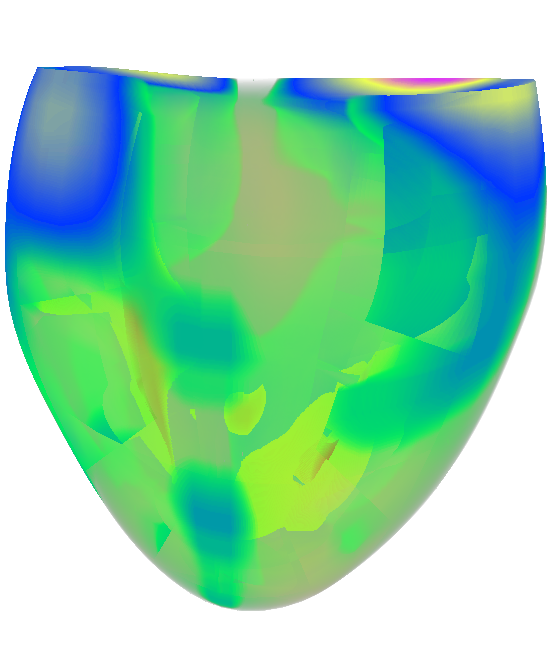
\includegraphics[width=0.4\linewidth]{figures/heart-2}
    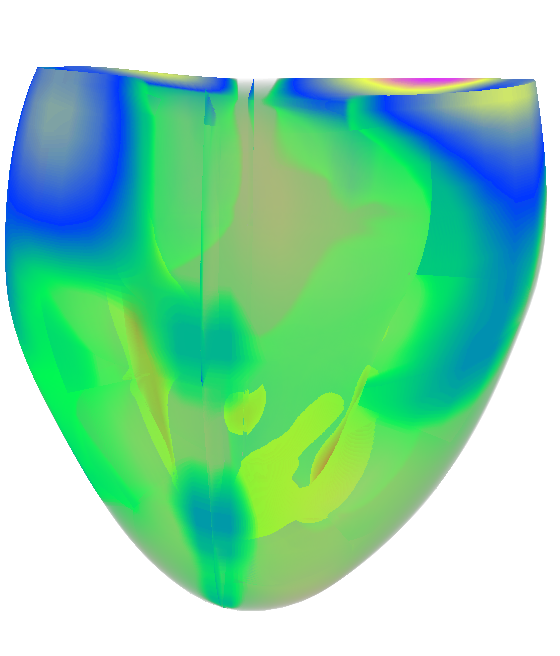
\includegraphics[width=0.4\linewidth]{figures/heart-2-rr-ii}}\\
    \subfigure[$10 \times 10$ precomputed proxy rays per element]{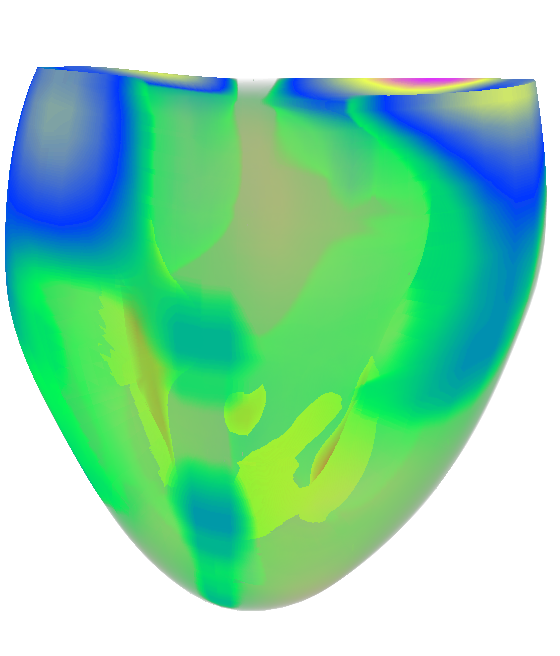
\includegraphics[width=0.4\linewidth]{figures/heart-10}
    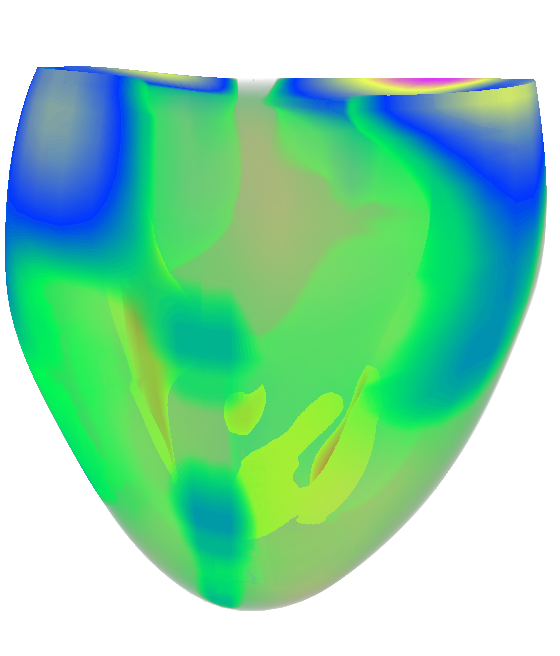
\includegraphics[width=0.4\linewidth]{figures/heart-10-rr-ii}}
    \caption{Application of our approach with different precomputation and rendering parameters. In the two rows, $2 \times 2$ ({\it a}) and $10 \times 10$ proxy rays ({\it b}) have been precomputed per element. Within each row, we show the application of standard ray-casting ({\it left}) as well as the proposed intra- and inter-ray interpolation scheme ({\it right}). \textbf{TODO: show closeups, does intra-ray interpolation make sense for the same entry exit resolution (?)(!!!).}}
    \label{fig:rayinterpolation}
\end{figure}

In order to further improve the image quality of our ray-casting approach, we introduce two specialized interpolation schemes: inter-ray interpolation and intra-ray interpolation. With the inter-ray interpolation, we use the four nearest proxy rays  instead of the proxy ray for a given pixel position, and interpolate between them. This interpolation is carried out by using bilinear interpolation at every sample position along the ray. The interpolation factors for these bilinear interpolations continuously vary along the ray, based on the factors derived for the entry and the exit face. The intra-ray interpolation instead, employs swapping of entry and exit points in order to obtain a mirrored copy of the current ray. Thus, we can interpolate between the original ray at position $t$ and the mirrored ray at position $t'=1-t$ while traversing the initially obtained ray. \textbf{TODO: does intra-ray interpolation make sense for the same entry exit resolution (?)(!!!).} Both of these interpolation schemes improve the image quality, as we show in Figure~\ref{fig:rayinterpolation}.

\section{Results}\label{sec:results}

\textbf{TODO: rewrite section.} To assess the quality and the performance of the proposed visualization technique, we have applied it to different data sets. Below, we will discuss the visual results, the introduced errors as well as the performance of our approach.

\subsection{Visual Results}

\begin{figure}[t]
    \centering 
    \subfigure[surface rendering]{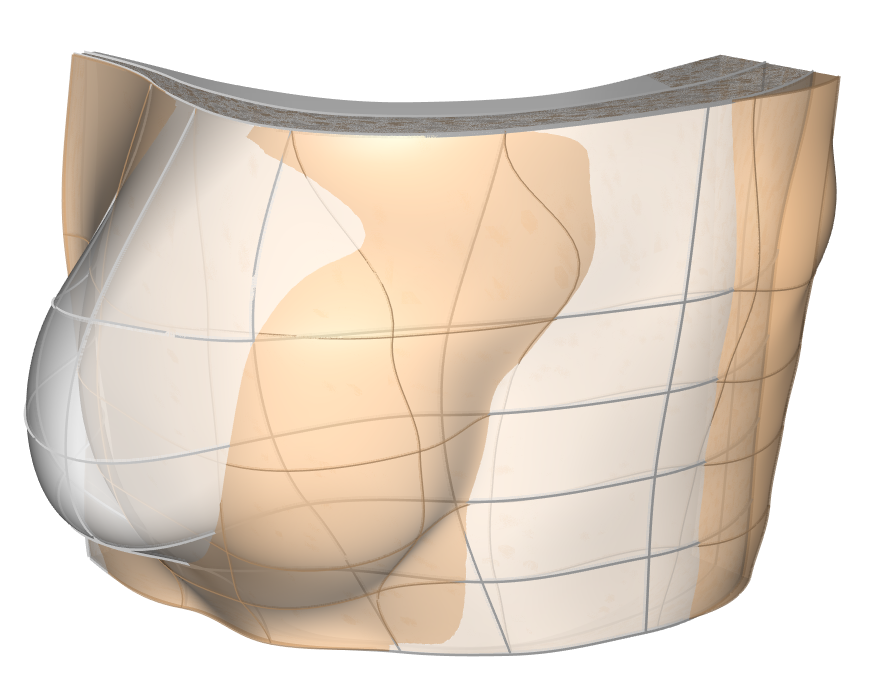
\includegraphics[width=0.45\linewidth]{figures/fem-breast}}
    \subfigure[volumetric rendering]{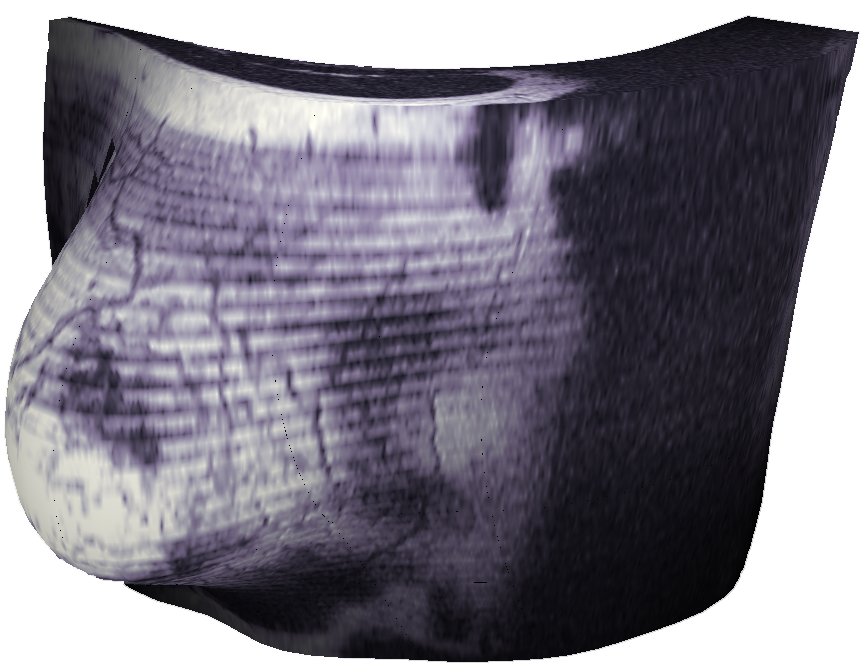
\includegraphics[width=0.45\linewidth]{figures/Breast}}
    \caption{FE breast model with MRI material space rendered as surface representation showing the deformed and the undeformed surface ({\it a}), and showing the deformed volume with our interactive volumetric approach ({\it b}).}
    \label{fig:breast}
\end{figure}

\begin{figure}[b]
    \centering 
    \subfigure[polygonal rendering]{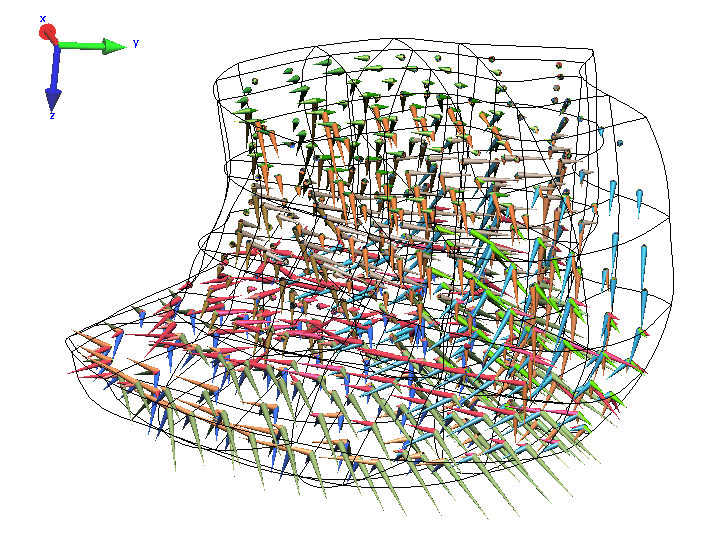
\includegraphics[width=0.45\linewidth]{figures/fem-tongue}}
    \subfigure[volumetric rendering]{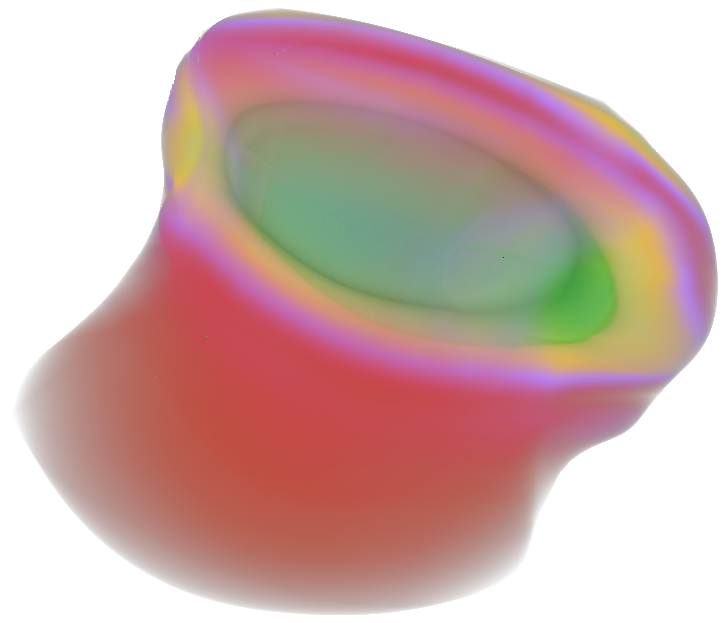
\includegraphics[width=0.45\linewidth]{figures/fem-tongue-new}}
    \caption{FE tongue model rendered as a polygonal representation ({\it a}), with our interactive volumetric approach ({\it b}).}
    \label{fig:tongue}
\end{figure}


\noindent \textbf{Breast model.} As the most simple model, we have applied our approach to a deformation model of a breast data set acquired from an MRI scan. The dependent variables in this case are the actual intensities of the MRI field, and the FE modeling has been applied to predict the supine shape of the data set originally acquired in the prone position. Figure~\ref{fig:breast} shows a comparison of the supine position rendered with our interactive volumetric approach ({\it b}) as compared to a standard surface based representation ({\it a}).

\noindent \textbf{Tongue model.} Furthermore, we have applied our approach to a model of a human tongue with simulated tissue densities and muscle fiber directions. In this case, each node stores one coordinate vector and seven derivatives and mixed derivatives for the tensor product of the cubic Hermite interpolation functions in all three coordinate directions. The results as compared to a polygonal representation are shown in Figure~\ref{fig:tongue}. Especially in this case, the multi-parametric capabilities of our algorithm are beneficial, as the tongue model contains 13 parameters. When instead, one would apply resampling to all of these parameter volumes, this would result in an unmanageable amount of data.

\noindent \textbf{Heart model.} A heart data set, where the strain values for each point have been computed from displacement values obtained from tagged MRI data, serves as the third example (see Figure~\ref{fig:heart}). Since the computation of the strain values was performed over the FE geometry, but using a numerical optimization technique, the strain values are represented as $11 \times 11 \times 6$ regular grids in material space, which are trilinearly interpolated. For our visualization, we have taken into account the three principal strain directions, which are the eigenvalues of the tensor. The principle strains include the maximum and minimum deformation and the corresponding eigenvectors give the direction of these deformations. These directions are circumferential, longitudinal and radial.

\begin{figure}[t]
    \centering 
		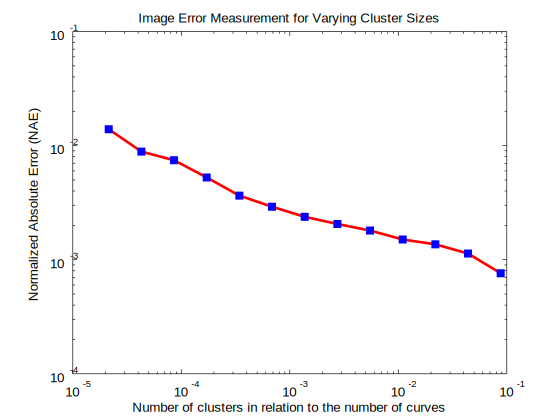
\includegraphics[width=0.8\linewidth]{figures/cluster_measurements/heart3/clusterErrorPlot}
    \caption{The normalized absolute pixel error (background pixels are neglected) plotted against the percentage of clusters relative to the total amount of curves.}
    \label{fig:clustering_visual_error}
\end{figure}


\subsection{Error Analysis}\label{subsec:error}
Our approach contains several steps which introduce potential errors. First, the proxy ray generation explained in Subsection~\ref{subsec:proxyraygeneration} introduces an error based on the number of actual proxy rays. The visual impact of this error is shown in Figure~\ref{fig:heart-analysis}. A second error is $\epsilon_{cluster}$ is the error introduced by the clustering scheme itself. Figure~\ref{fig:clustering_epsilon_error} shows the error for a varying number of clusters. It is clear, that the error becomes smaller if we use more clusters. The number of clusters can, depending on data set, be quite low in relation to the number of splines, as seen in Figure~\ref{fig:clustering_visual_error}. This is due to the fact that clustering of the curves is performed without consideration for the angle, as this stored in separately, which increase the correlation between the curves.

\subsection{Performance Analysis}\label{subsec:performance}

\begin{figure}[t]
    \centering 
    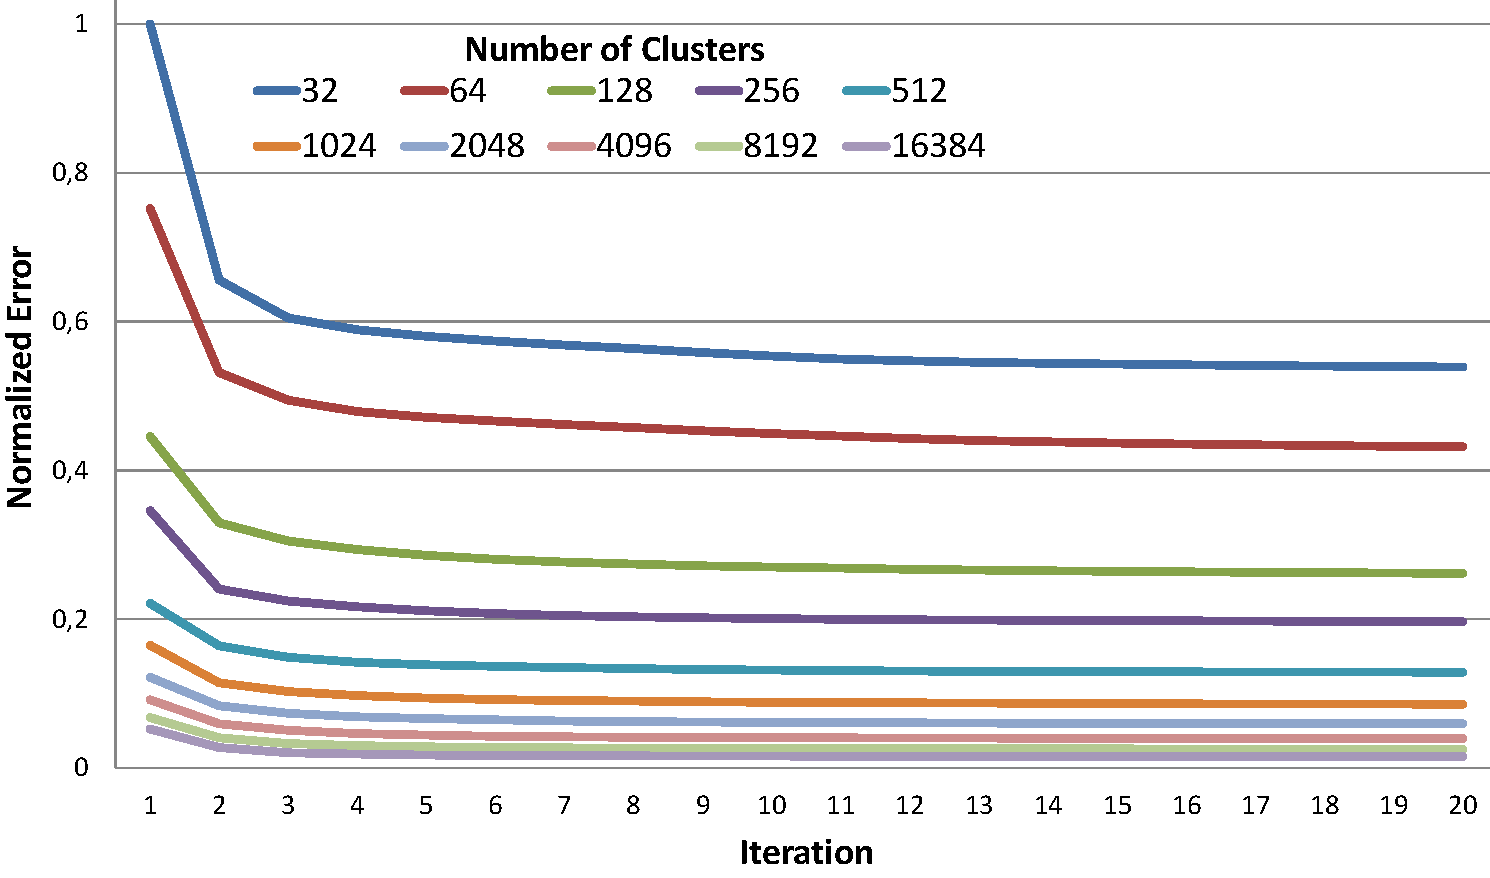
\includegraphics[width=0.85\linewidth]{figures/diagram_num_clusters}
    \caption{The error for varying numbers of clusters in depending on the number of iterations after which the k-means algorithm has stopped. The data is based on the heart data set with a grid resolution of $5\times5$, which resulted in 360.000 rays. Initial error for 32 clusters has the value 1.}
    \label{fig:clustering_epsilon_error}
\end{figure}

\begin{table}[t]
  \caption{Performance analysis (in fps) of our technique for different grid sizes compared to GPU FHP implementation(visualizing only first hit point, i.\,e., no transparency).}
  \label{tab:performance}
  \begin{center}
    \begin{tabular}{|l|c|c|c|c|c|c|}
      \hline
      Pixel & GPU & \multicolumn{5}{c|}{Our Technique}\\
      Res & (FHP) & $2^2$ & $3^2$ & $4^2$ & $6^2$ & $10^2$ \\
      \hline
      $768^2$ & 7.51 & 15.60 & 15.36 & 15.21 & 15.33 & 15.20\\
      $1280^2$ & 4.19 & 10.70 & 10.51 & 10.31 & 10.26 & 10.24\\
      \hline
    \end{tabular}
  \end{center}
\end{table}


We have to differentiate between the precomputation and the rendering step in the performance analysis. Although, the time used for precomputation is dependent on both the proxy ray computation and the clustering, the latter takes more time than the former. In our unoptimized CPU implementation, the clustering for a $5\times5$ grid with $8192$ clusters takes roughly 4-6 hours, while a $15\times15$ grid with $8192$ clusters takes approximately 72-84 hours of time. The measurement have such a high degree of deviation because the machine the test ran on was used lightly during the computation. In the future we would like to increase the precomputation time by exploiting a GPU architecture implementation, which has could increase the clustering speed in a very similar application case by a factor of ten~\cite{mess10gpuclustering}. Table \ref{tab:performance} shows the rendering performance of our interactive volumetric technique compared to a first hit GPU implementation performing no ray marching and thus not allowing volumetric rendering with transparency. \textbf{TODO: discuss texture sizes.}



\section{Conclusions \& Future Work}\label{sec:conclusions}
In this paper we have presented a ray-casting based approach which allows the interactive exploration of FE models. By shifting the computationally complex world to $\xi$ space transformation from the rendering stage into a preprocessing stage, we are able to achieve interactive frame rates and thus allow an interactive in-detail inspection of FE models on standard GPUs. To our knowledge, this is the first approach, allowing an interactive true volumetric exploration of curvilinear FE models. We have demonstrated the outcome of the presented approach by applying it to several real-world data sets from different disciplines, and by analyzing the errors introduced by our approach.

In the future, there are several opportunities to further improve the presented concepts. When precomputing the proxy rays, we currently use a equidistant layout for the generation of the set $P$ of uniformly distributed start and end points. Here it could be explored, how other layouts borrowed for instance from ray sampling as described in the computer graphics literature, could further improve quality. In the preprocessing step, especially the clustering takes a long time, due to the high number of precomputed proxy rays. Hence, this preprocessing could be optimized by utilizing programming techniques for parallel architectures. While, our approach currently supports scalar data only, in the future we plan to use the proposed method to visualize vector and tensor data defined over $\xi$ space.


\bibliographystyle{abbrv}
\bibliography{literature-fem}

\end{document}